\documentclass[../notes.tex]{subfiles}

\pagestyle{main}
\renewcommand{\chaptermark}[1]{\markboth{\chaptername\ \thechapter\ (#1)}{}}
\setcounter{chapter}{5}

\begin{document}




\chapter{Cations}
\setcounter{section}{32}
\section{Cations}
\begin{itemize}
    \item \marginnote{11/25:}Lecture 32 recap.
    \begin{itemize}
        \item Claisen condensations provide 1,3-dicarbonyls (Figure \ref{fig:claisenCondensation}).
        \begin{itemize}
            \item Remember that we need two hydrogens to deprotonate!
            \item These reactions proceed under 1 equivalent of base.
            \item Driving force: Formation of the enolate.
            \item Workup yields the final 1,3-dicarbonyl, also known as a $\beta$-dicarbonyl.
        \end{itemize}
        \item Michael reactions provide 1,5-dicarbonyls (Figure \ref{fig:michael}).
        \begin{itemize}
            \item We mostly discussed carbonyl enolates, sometimes from $\beta$-dicarbonyls!
        \end{itemize}
    \end{itemize}
    \item Today: We'll begin Unit 6 (carbocations).
    \begin{itemize}
        \item The beginning of this unit is a recap of what you already know about carbocations.
        \begin{itemize}
            \item Review your 5.12 notes!!
            \item And/or read \textcite[333-339]{bib:Clayden}.
            \item We'll cover Chapter 36 of \textcite{bib:Clayden} toward the end of this unit.
        \end{itemize}
        \item Aside (history): Carbocations were called "carbocations" when Prof. Buchwald was in school, then "carbenium ions" for a time, and now are known as "carbocations" again.
    \end{itemize}
    \item Lecture outline.
    \begin{enumerate}[label={\Alph*.}]
        \item Introduction to carbocations.
        \item Generating carbocations.
        \begin{enumerate}[label={\arabic*)}]
            \item Addition of an electrophile to a multiple bond.
            \item Heterolytic cleavage of \ce{C-X} bonds.
        \end{enumerate}
        \item Reactions.
        \begin{enumerate}[label={\arabic*)}]
            \item Eliminations.
            \item Combinations with nucleophiles.
            \begin{enumerate}[label={\alph*)},start=2]
                \item Reactions with aromatic rings.
                \begin{itemize}
                    \item Friedel-Crafts alkylation.
                    \item Friedel-Crafts acylation.
                \end{itemize}
                \item Reactions with olefins.
            \end{enumerate}
            \item Rearrangements and fragmentations.
            \begin{itemize}
                \item Friedel-Crafts alkylation (revisited).
            \end{itemize}
        \end{enumerate}
    \end{enumerate}
    \item We'll begin with Topic A: Introduction to carbocations.
    \item \textbf{Carbocation}: A species that contains a carbon bearing a positive charge. \emph{Structure}
    \begin{figure}[H]
        \centering
        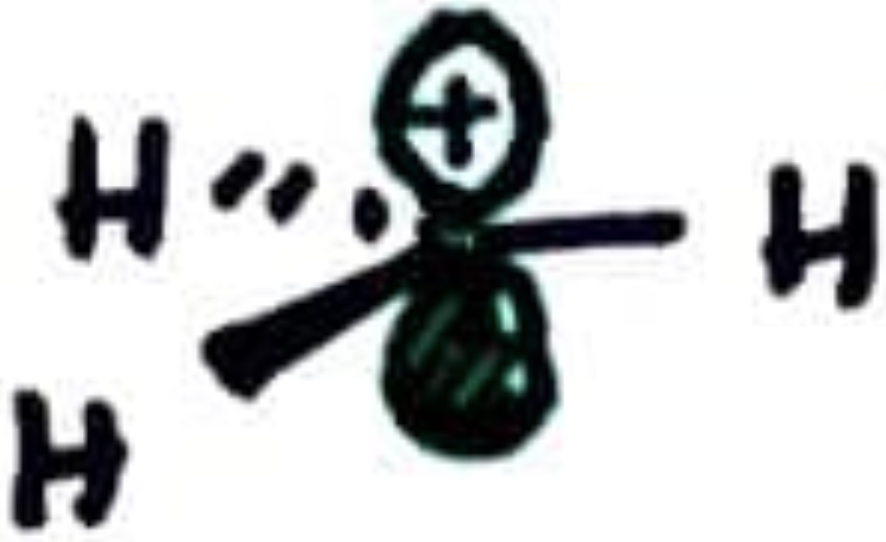
\includegraphics[width=0.1\linewidth]{CC.png}
        \caption{Carbocation.}
        \label{fig:CC}
    \end{figure}
    \begin{itemize}
        \item These are $sp^2$-hybridized species, so typically with three \ang{120} bond angles.
        \item However, carbocation bond angles can be strained in rings, for example.
    \end{itemize}
    \item Stabilizing cations.
    \begin{figure}[h!]
        \centering
        \begin{subfigure}[b]{0.3\linewidth}
            \centering
            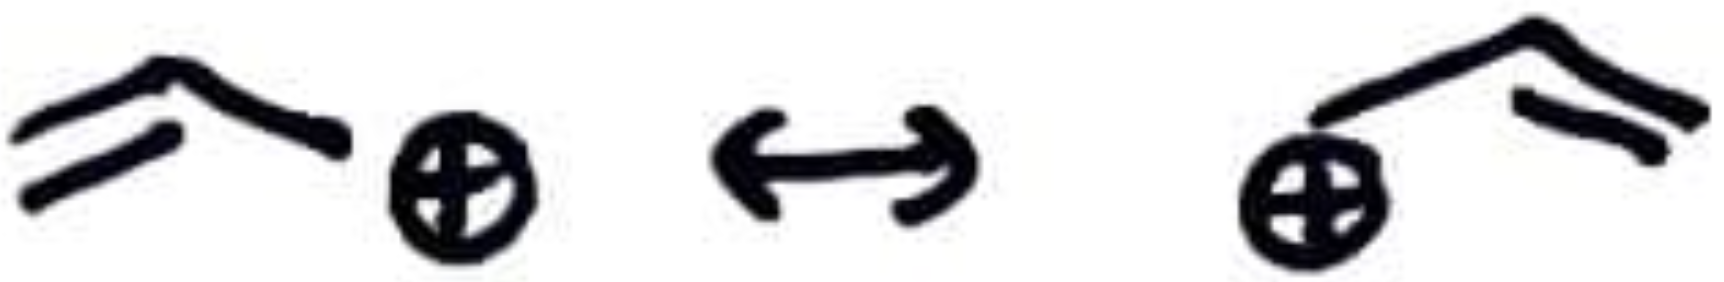
\includegraphics[width=0.8\linewidth]{CCstablea.png}
            \caption{Allyl cation.}
            \label{fig:CCstablea}
        \end{subfigure}
        \begin{subfigure}[b]{0.3\linewidth}
            \centering
            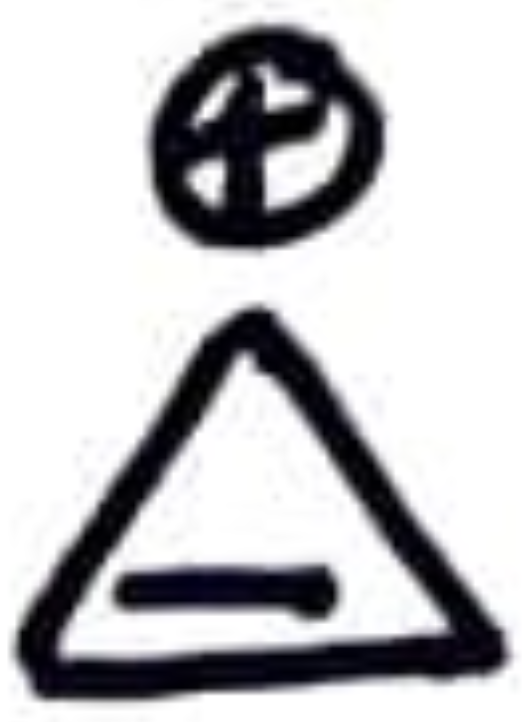
\includegraphics[width=0.15\linewidth]{CCstableb.png}
            \caption{Cyclopropenyl cation.}
            \label{fig:CCstableb}
        \end{subfigure}
        \caption{Stabilized carbocations.}
        \label{fig:CCstable}
    \end{figure}
    \begin{itemize}
        \item The allyl cation is stabilized by resonance.
        \item The cyclopropenyl cation is stabilized by $4(0)+2=2\pi$ electron H\"{u}ckel aromaticity, even though it has significant angle strain ($\ang{120}\to\ang{60}$).
    \end{itemize}
    \item Heteroatom-stabilized carbocations are good.
    \begin{figure}[h!]
        \centering
        \begin{subfigure}[b]{0.33\linewidth}
            \centering
            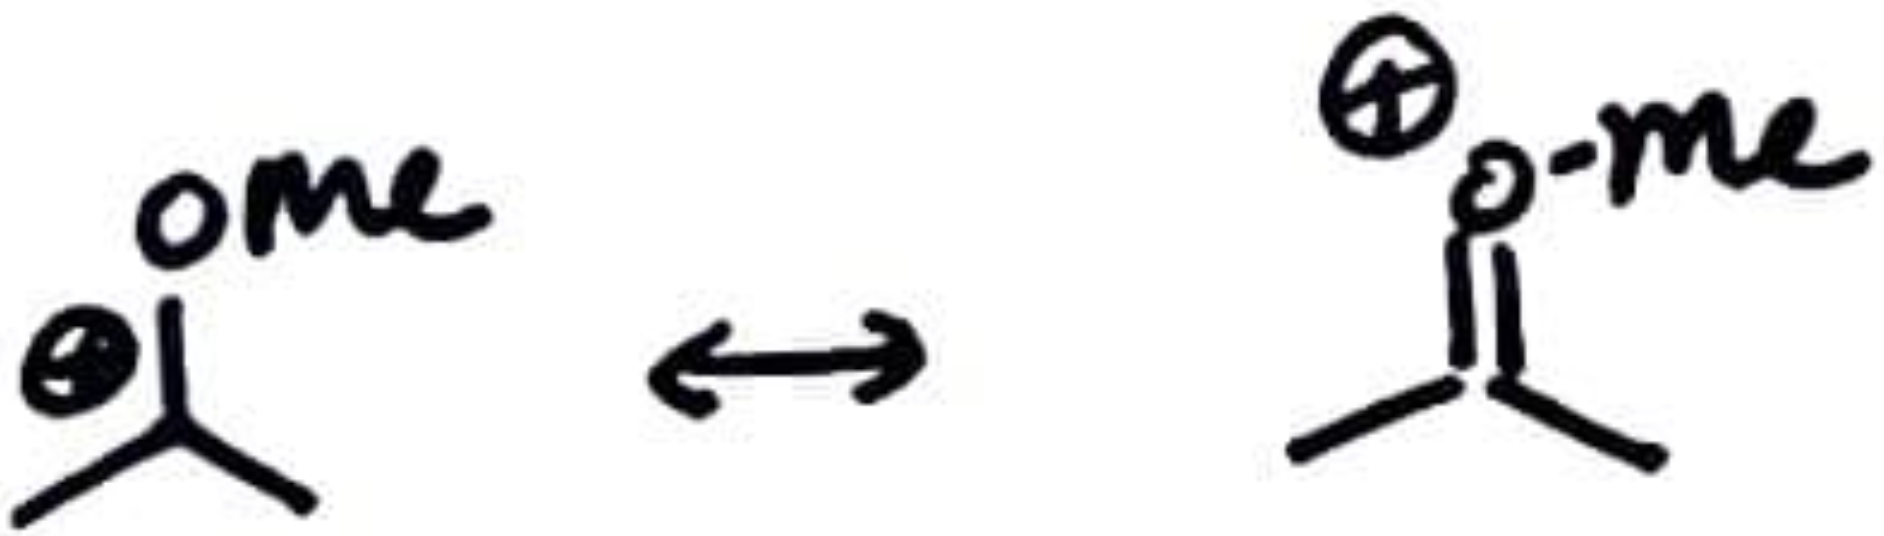
\includegraphics[width=0.8\linewidth]{CCheteroatoma.png}
            \caption{Oxocarbenium ion.}
            \label{fig:CCheteroatoma}
        \end{subfigure}
        \begin{subfigure}[b]{0.32\linewidth}
            \centering
            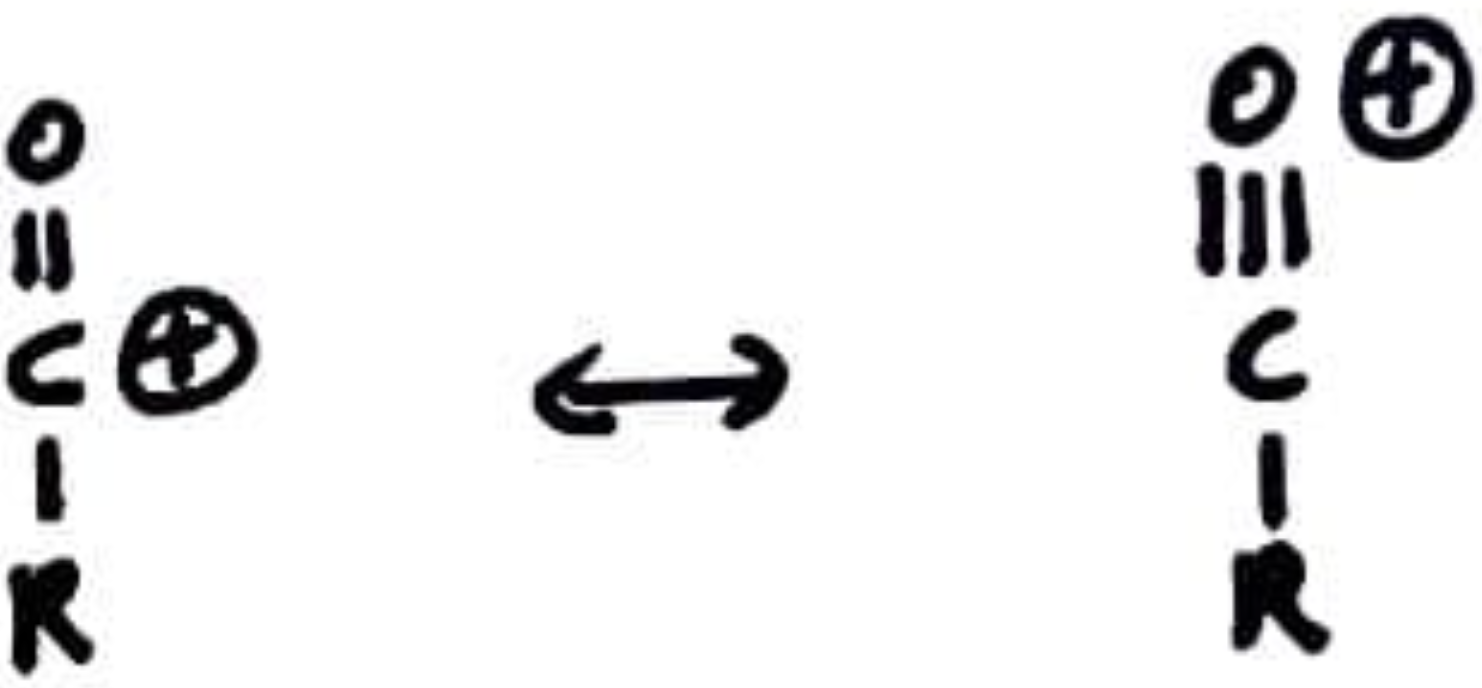
\includegraphics[width=0.65\linewidth]{CCheteroatomb.png}
            \caption{Acylium ion.}
            \label{fig:CCheteroatomb}
        \end{subfigure}
        \begin{subfigure}[b]{0.33\linewidth}
            \centering
            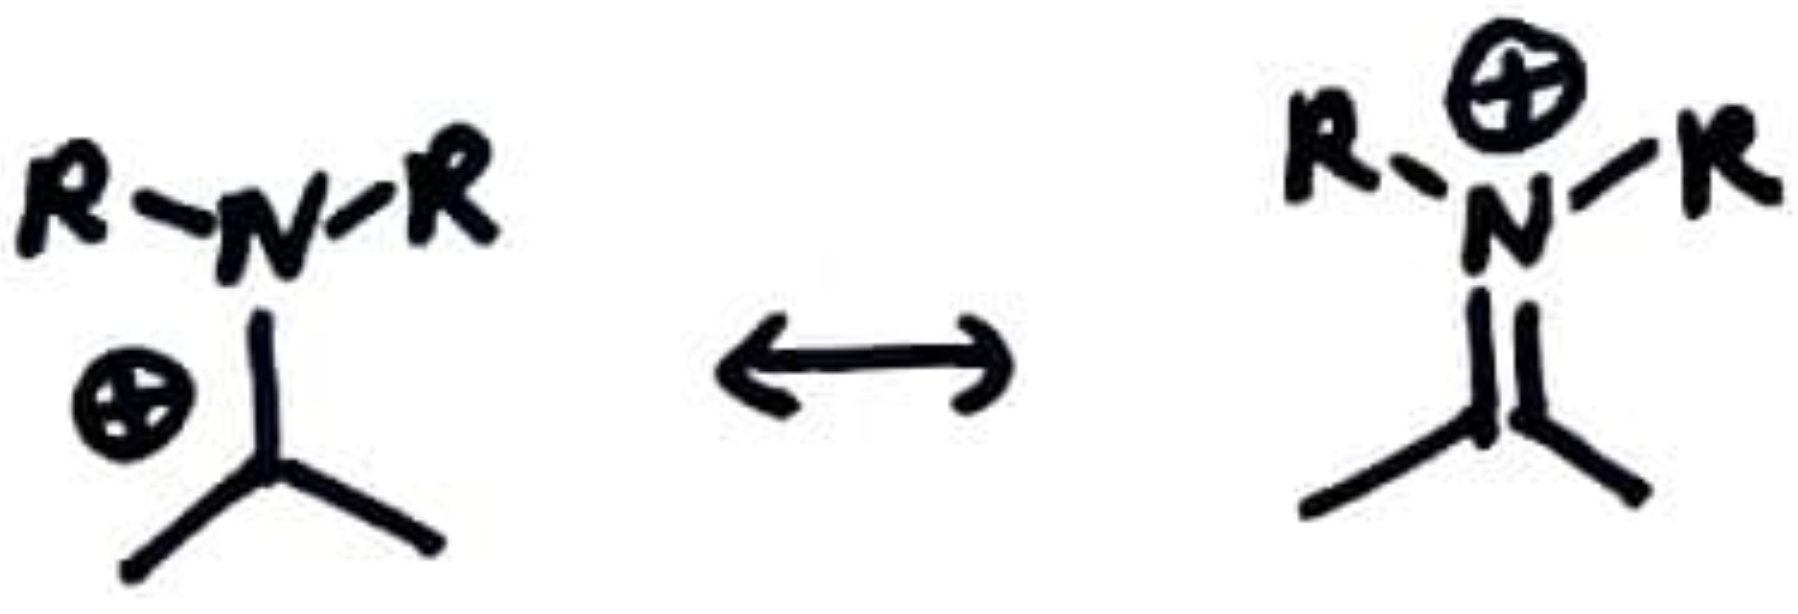
\includegraphics[width=0.75\linewidth]{CCheteroatomc.png}
            \caption{Iminium ion.}
            \label{fig:CCheteroatomc}
        \end{subfigure}
        \caption{Heteroatom-stabilized carbocations.}
        \label{fig:CCheteroatom}
    \end{figure}
    \begin{itemize}
        \item Figure \ref{fig:CCheteroatoma} depicts an intermediate in the hydrolysis of ketals.
        \item Heteroatom-stabilized cations can have synthetic utility, e.g., the acylium ion present in the mechanism of Friedel-Crafts acylations.
        \item Iminium ions are also technically heteroatom-stabilized carbocations.
    \end{itemize}
    \item Ordering carbocation stability.
    \begin{equation*}
        \text{benzyl} > \text{allyl} > 3^\circ > 2^\circ > 1^\circ > \ce{Me} > \text{vinyl} > \text{phenyl}
    \end{equation*}
    \begin{itemize}
        \item $1^\circ$, methyl, vinyl, and phenyl cations will not be discussed further in 5.13.
        \begin{itemize}
            \item Possible exception: Know that they exist, and that they're bad.
        \end{itemize}
        \item Benzyl cations are stabilized by significant resonance delocalization of their positive charge.
        \begin{itemize}
            \item This resonance implies that the \emph{ortho}- and \emph{para}-positions have $\delta^+$ charges on them.
            \item Thus, substitutions at these positions affect carbocation stability!
            \item Example: Compare the relative stability of the \emph{para}-trifluoromethylbenzyl cation, \emph{para}-methylbenzyl cation, and \emph{para}-methoxybenzyl cation.
            \begin{itemize}
                \item Trifluoromethyl is a destabilizing EWG, methyl is an inductively stabilizing EDG, and methoxy is a resonance stabilizing EDG.
            \end{itemize}
        \end{itemize}
        \pagebreak
        \item Allyl is good; any time we can add additional resonance forms \emph{of the same energy}, we get stabilization.
        \item More substituted carbocations are stabilized by hyperconjugation (see Figure \ref{fig:hyperconjugationCC}).
        \begin{itemize}
            \item Recall that such resonance structures are sometimes referred to as "no-bond resonance forms."
            \item No-bond resonance structures are ok because they do not violate the fundamental principle that \emph{atoms must not move between resonance structures}.
            \begin{itemize}
                \item This is a very easy thing to forget, for intro students up to tenured professors at MIT! So be careful!!
            \end{itemize}
            \item The active mode of stabilization here is $\sigma$-donation.
        \end{itemize}
    \end{itemize}
    \item We now move onto Topic B: Generating carbocations.
    \item We'll begin with Subtopic B.1: Addition of an electrophile to a multiple bond.
    \begin{figure}[h!]
        \centering
        \begin{subfigure}[b]{0.45\linewidth}
            \centering
            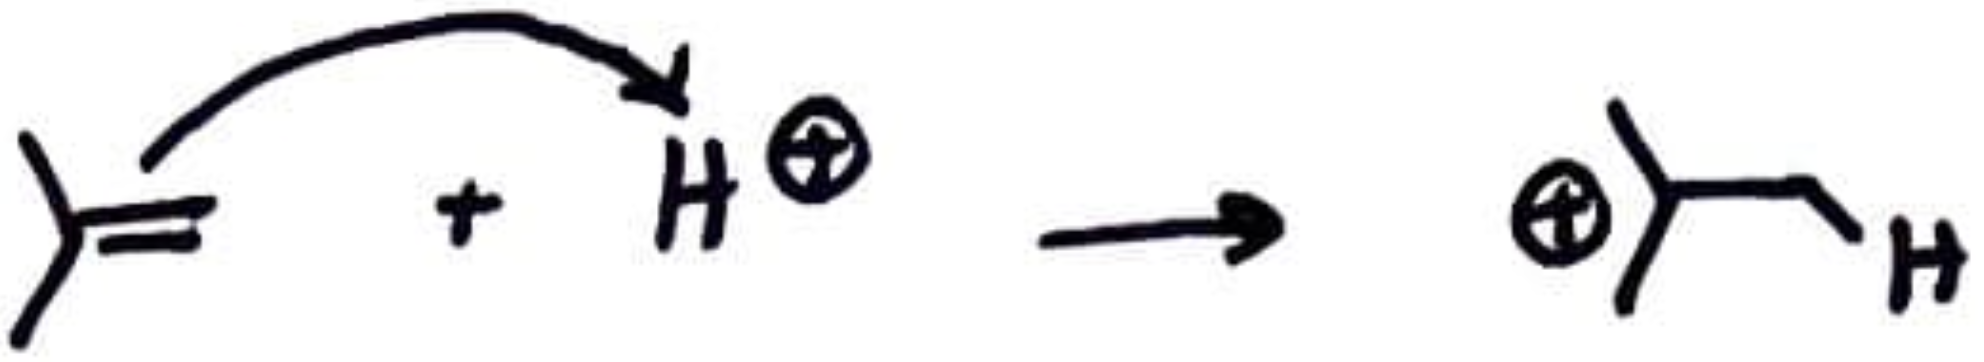
\includegraphics[width=0.7\linewidth]{CCmultiplea.png}
            \caption{Markovnikov addition to an olefin.}
            \label{fig:CCmultiplea}
        \end{subfigure}
        \begin{subfigure}[b]{0.45\linewidth}
            \centering
            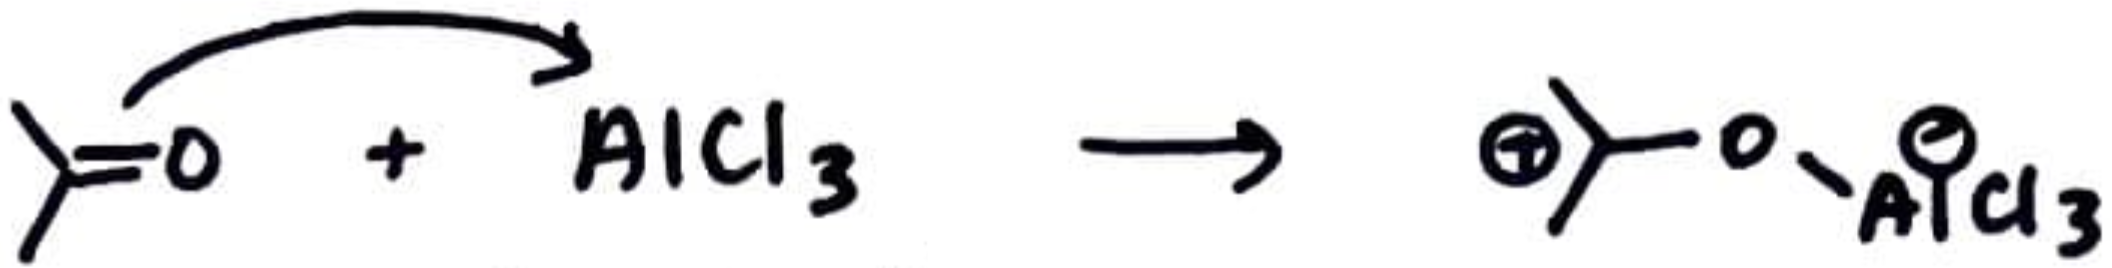
\includegraphics[width=0.95\linewidth]{CCmultipleb.png}
            \caption{Lewis acid coordination.}
            \label{fig:CCmultipleb}
        \end{subfigure}
        \caption{Multiple bonds can cleave to generate carbocations.}
        \label{fig:CCmultiple}
    \end{figure}
    \begin{itemize}
        \item We protonate in accordance with \textbf{Markovnikov's rule}.
        \item Additionally, just like silicon is \textbf{oxophilic}, aluminum is an oxophilic Lewis acid.
    \end{itemize}
    \item \textbf{Markovnikov's rule}: Protonate so as to generate the most highly-substituted carbocation.
    \item \textbf{Oxophilic} (element): An element that has a strong affinity for binding to oxygen. \emph{Etymology} from Latin "lover of oxygen."
    \item We now move onto Subtopic B.2: Heterolytic cleavage of \ce{C-X} bonds.
    \begin{figure}[h!]
        \centering
        \begin{subfigure}[b]{\linewidth}
            \centering
            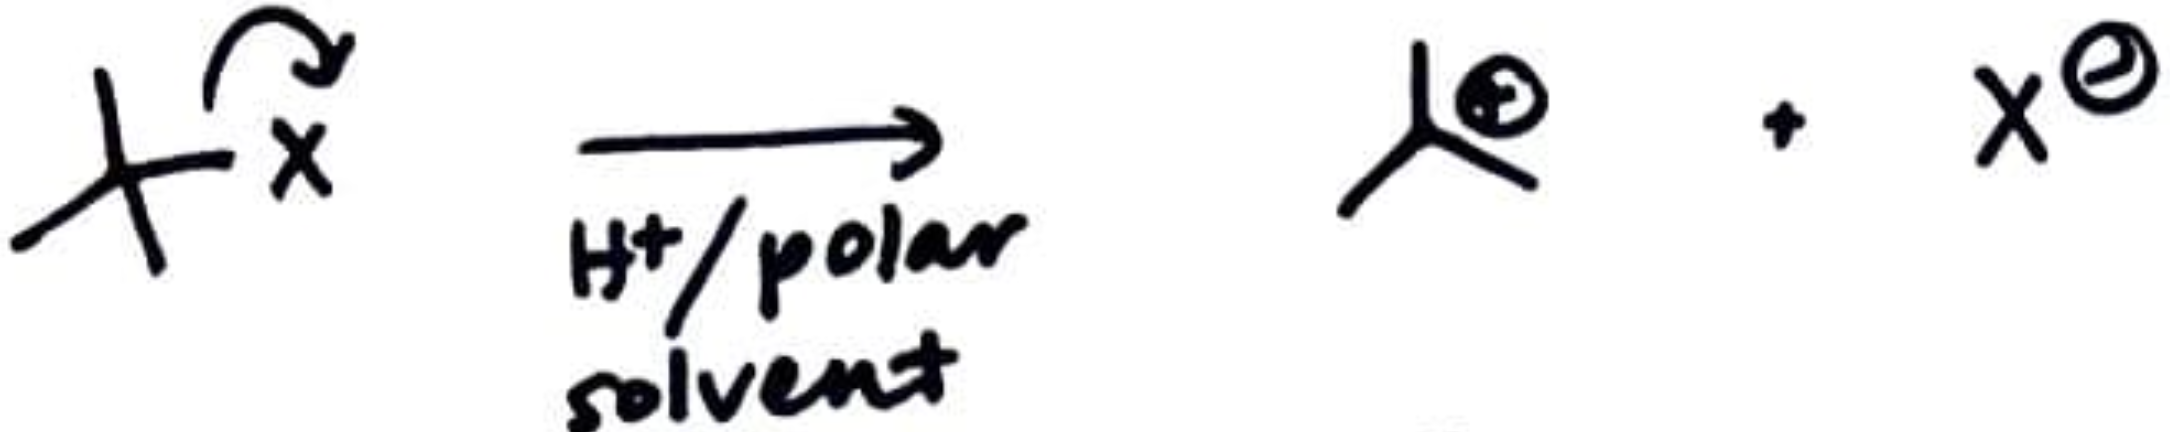
\includegraphics[width=0.4\linewidth]{CCheteroCleavea.png}
            \caption{General form.}
            \label{fig:CCheteroCleavea}
        \end{subfigure}\\[2em]
        \begin{subfigure}[b]{\linewidth}
            \centering
            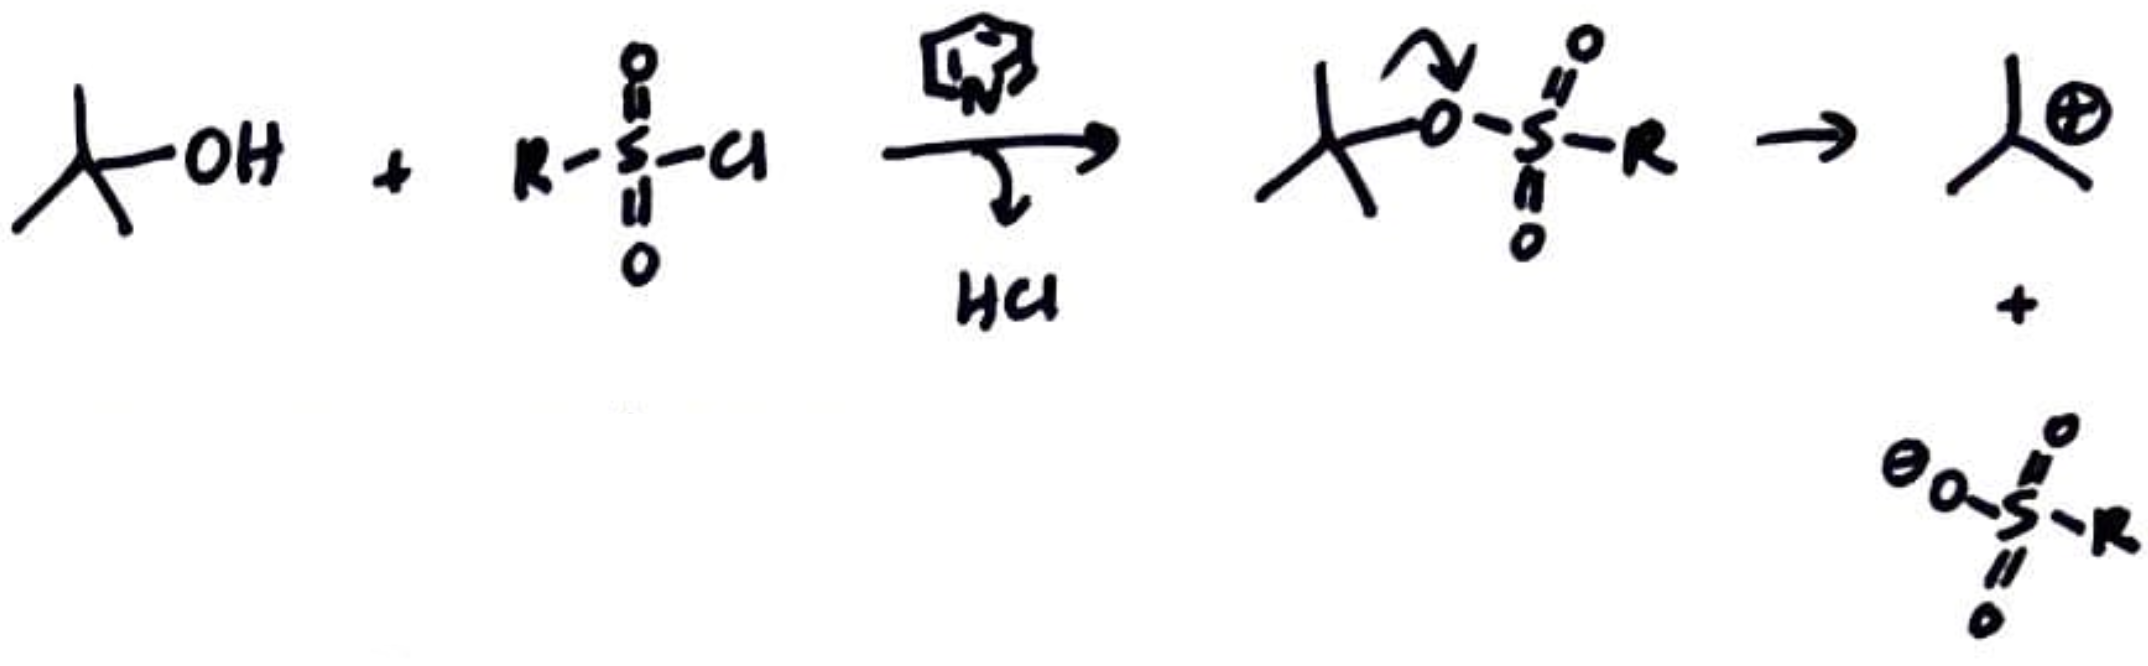
\includegraphics[width=0.6\linewidth]{CCheteroCleaveb.png}
            \caption{Sulfonate leaving groups.}
            \label{fig:CCheteroCleaveb}
        \end{subfigure}
        \caption{Generating carbocations from heterolytic \ce{C-X} bond cleavage.}
        \label{fig:CCheteroCleave}
    \end{figure}
    \begin{itemize}
        \item Acid promotes the departure of the leaving group.
        \item We often run these reactions in polar solvents (e.g., DMF) to help stabilize the leaving group.
        \item If we make a sulfonate out of a tertiary alcohol (using base), this can then leave --- water, by itself, isn't a great leaving group.
    \end{itemize}
    \item What's to stop the leaving group from just reattacking the carbocation?
    \begin{itemize}
        \item It can! Leaving group departure is most certainly a reversible process.
        \item Leaving group departure is just a way to generate a carbocation if you have a reaction in mind \emph{other than} the transiently formed carbocation just reattracting the lone pair of the leaving group.
    \end{itemize}
    \item We now move onto Topic C: Reactions.
    \item We'll begin with Subtopic C.1: Eliminations.
    \begin{figure}[h!]
        \centering
        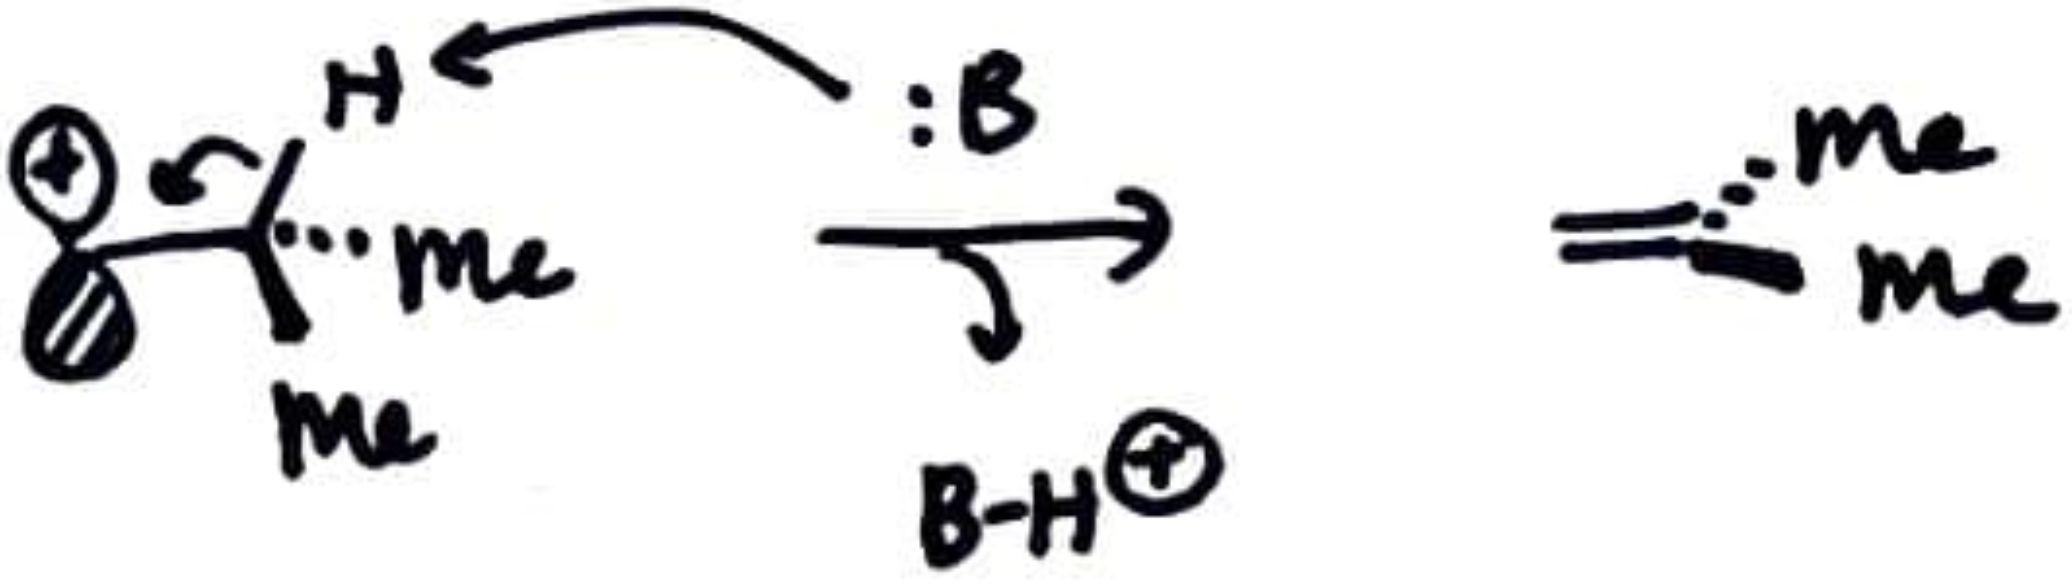
\includegraphics[width=0.35\linewidth]{CCelimE1.png}
        \caption{E\textsubscript{1} elimination of carbocations.}
        \label{fig:CCelimE1}
    \end{figure}
    \begin{itemize}
        \item This is the simplest carbocation reaction.
        \item This can be useful for isomerizing alkenes because you will preferentially eliminate to form the more substituted alkene.\footnote{The more substituted alkene is more stable per \textbf{Zaitsev's rule}.}
    \end{itemize}
    \item We now move onto Subtopic C.2: Combinations with nucleophiles.
    % \item We'll begin with Subtopic C.2.1: Reactions with lone pairs.
    \item We now move onto Subtopic C.2.b{}: Reactions with aromatic rings.
    \item Consider the reaction of benzene, \emph{t}-butyl chloride, and a Lewis acid (LA).
    \begin{figure}[h!]
        \centering
        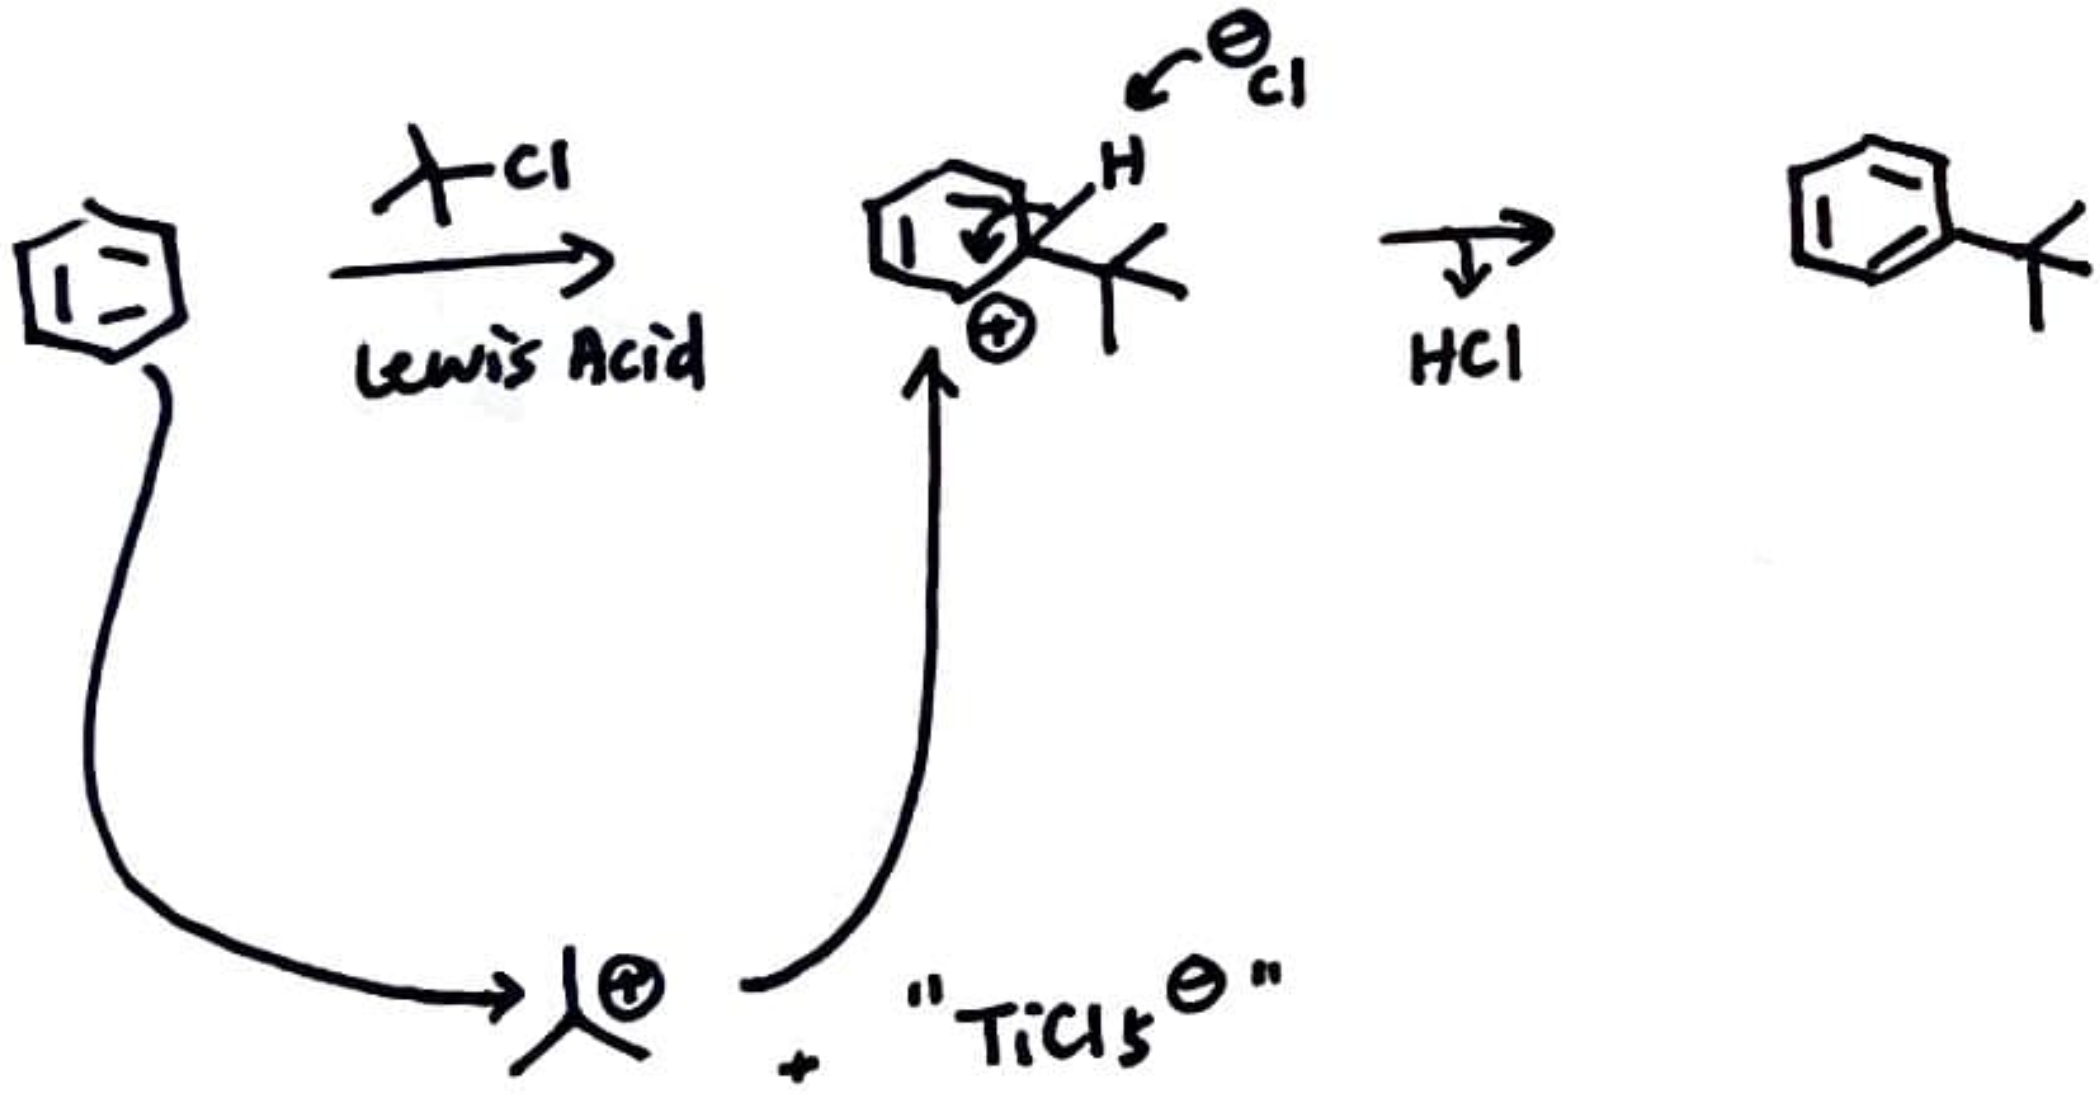
\includegraphics[width=0.5\linewidth]{FCalkyl.png}
        \caption{Friedel-Crafts alkylation.}
        \label{fig:FCalkyl}
    \end{figure}
    \begin{itemize}
        \item As an example of a Lewis acid, you can use titanium tetrachloride (\ce{TiCl4}).
        \begin{itemize}
            \item \ce{TiCl4} is chlorophilic, and wants to form the \ce{TiCl5-} adduct.
        \end{itemize}
        \item You can form a carbocation that will be attacked by benzene and then eliminated by chloride.
    \end{itemize}
    \item You can also form a cation from an alkene and then react that with benzene.
    \begin{figure}[H]
        \centering
        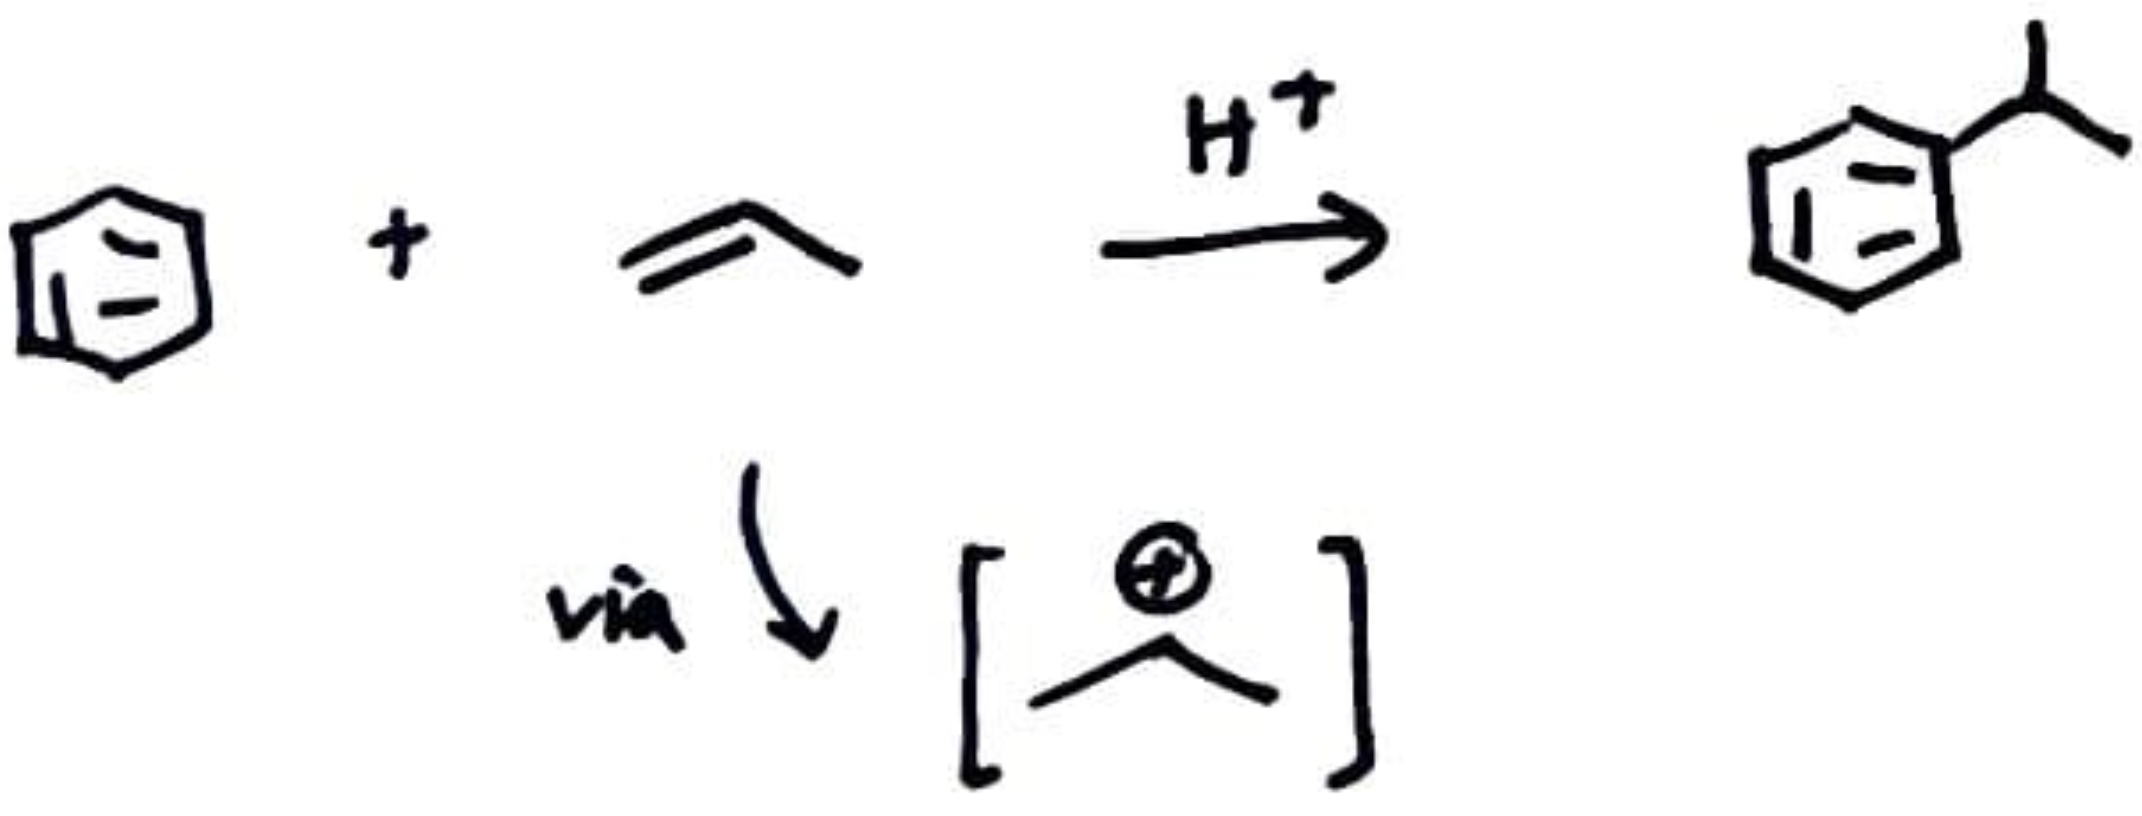
\includegraphics[width=0.45\linewidth]{Hock.png}
        \caption{Hock process (stage 1).}
        \label{fig:Hock}
    \end{figure}
    \begin{itemize}
        \item This is the primary method of producing acetone.\footnote{You can read more about this process --- called the \textbf{Hock process} --- on \href{https://en.wikipedia.org/wiki/Cumene_process}{Wikipedia}.}
        \item It astounds Prof. Buchwald that this is economical: Indeed, it's easier to attach the isopropyl group to benzene and then rip it apart again, then it is to convert it directly to acetone.
    \end{itemize}
    \item Friedel-Crafts acylation.
    \begin{figure}[h!]
        \centering
        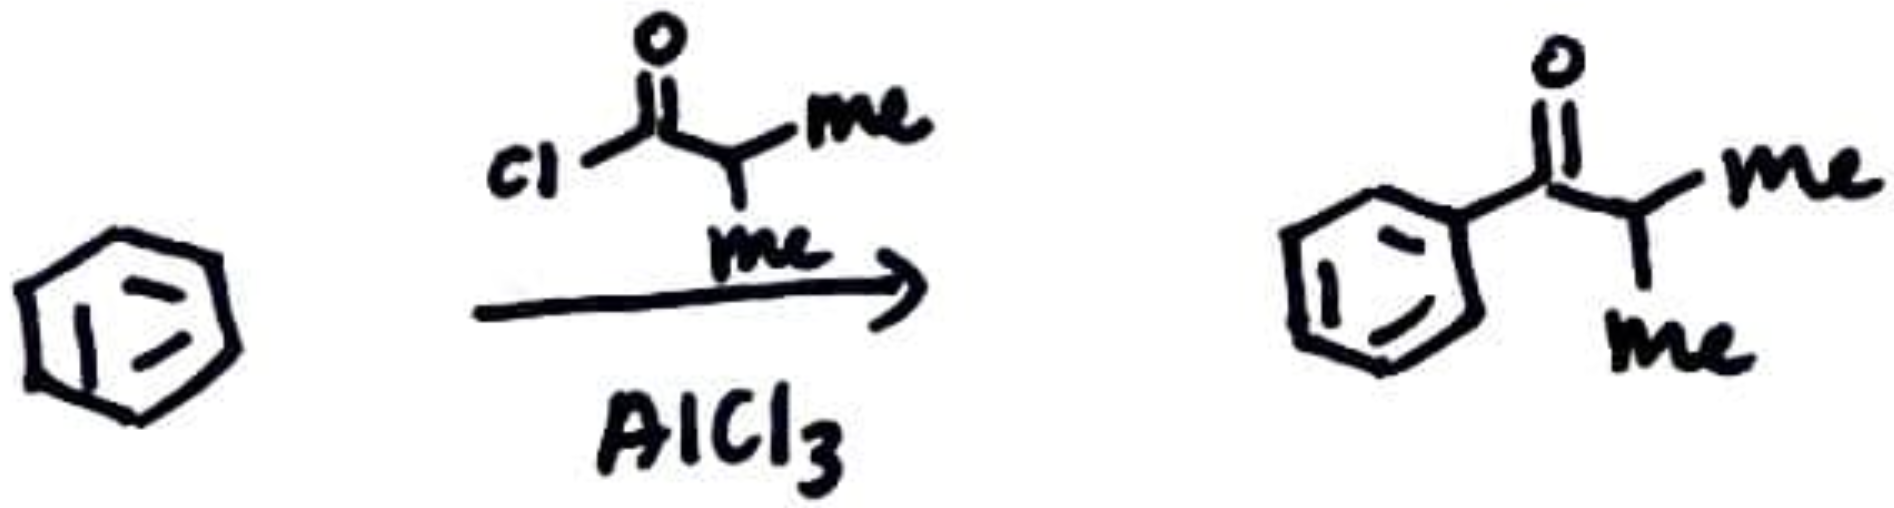
\includegraphics[width=0.4\linewidth]{FCacyl.png}
        \caption{Friedel-Crafts acylation.}
        \label{fig:FCacyl}
    \end{figure}
    \item Asides on Friedel-Crafts acylation.
    \begin{itemize}
        \item Crafts was the president of MIT at one point, once he got tired of running these reactions!
        \item If you open a bottle of \ce{AlCl3}, it reacts with water in the air to release \ce{HCl} (very toxic).
    \end{itemize}
    \item We now move onto Subtopic C.2.c{}: Reactions with olefins.
    \begin{figure}[h!]
        \centering
        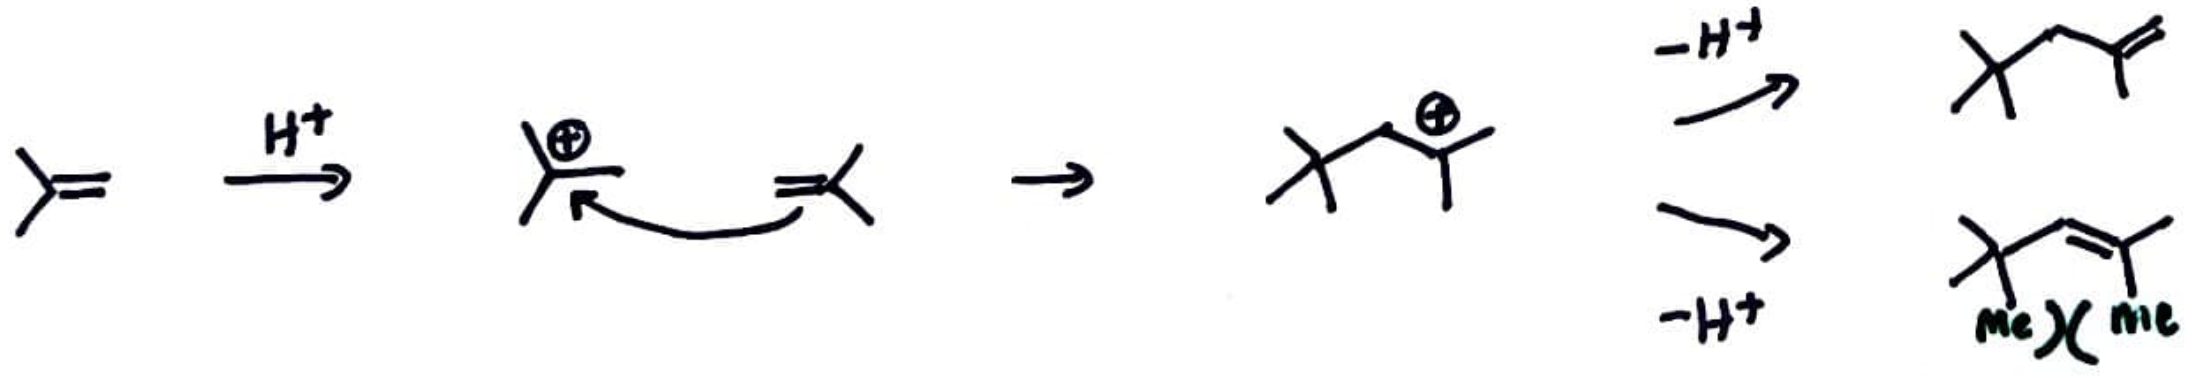
\includegraphics[width=0.9\linewidth]{CColefinDimer.png}
        \caption{Olefin dimerization via carbocations.}
        \label{fig:CColefinDimer}
    \end{figure}
    \begin{itemize}
        \item Dimerization under equilibrating conditions would give \emph{mostly} the trisubstituted olefin, but not $100:0$ because the trisubstituted olefin has some steric clash between the methyl and \emph{t}-butyl group. This steric clash raises its energy relative to the disubstituted alkene product.
    \end{itemize}
    \item We now move onto Subtopic C.3: Rearrangements and fragmentations.
    \begin{figure}[h!]
        \centering
        \begin{subfigure}[b]{\linewidth}
            \centering
            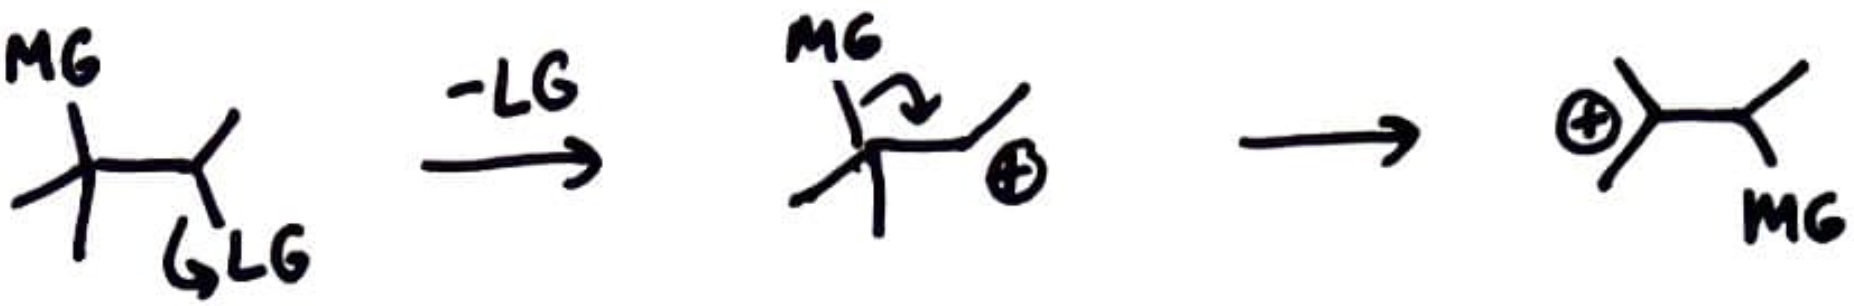
\includegraphics[width=0.55\linewidth]{CCrearra.png}
            \caption{Stepwise pathway.}
            \label{fig:CCrearra}
        \end{subfigure}\\[2em]
        \begin{subfigure}[b]{\linewidth}
            \centering
            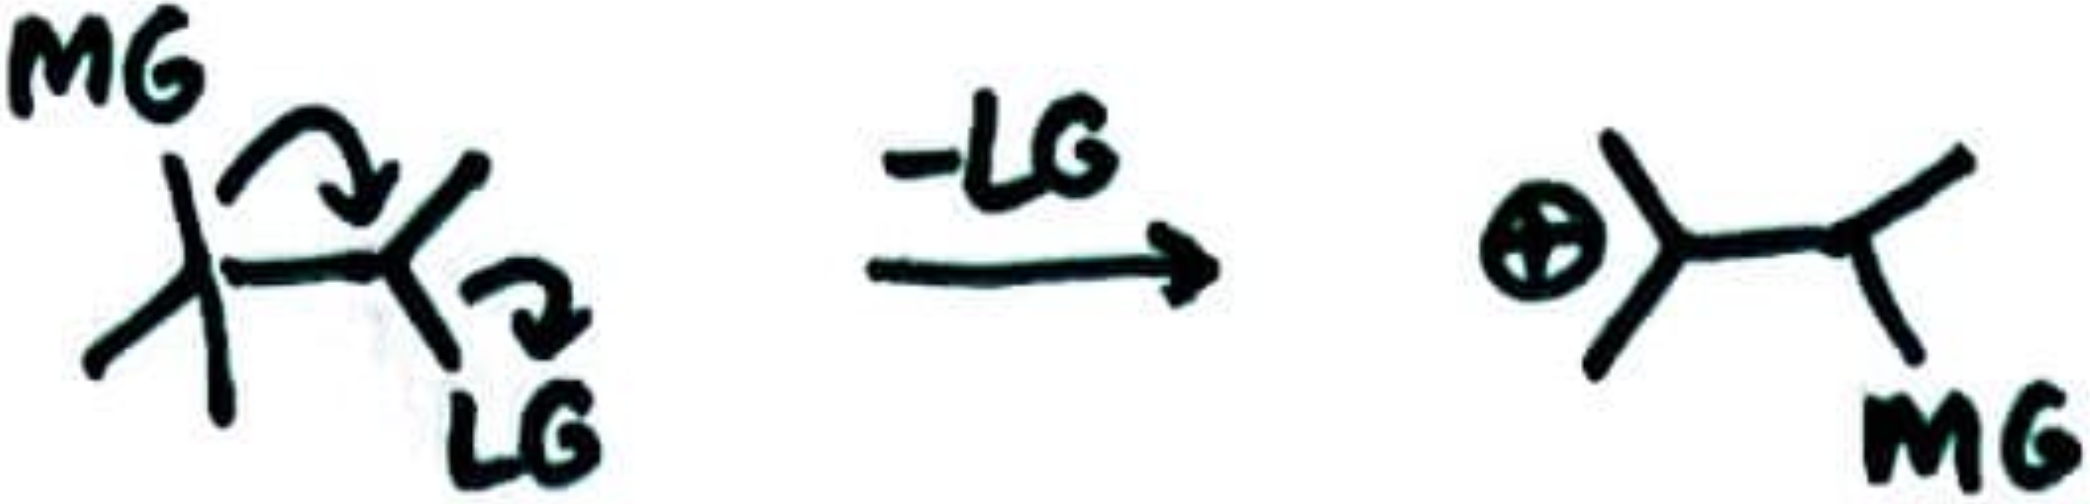
\includegraphics[width=0.3\linewidth]{CCrearrb.png}
            \caption{Concerted pathway.}
            \label{fig:CCrearrb}
        \end{subfigure}
        \caption{Carbocation rearrangement.}
        \label{fig:CCrearr}
    \end{figure}
    \begin{itemize}
        \item The \ce{MG} is the "migrating group," and the LG is the "leaving group."
        \item When the leaving group departs, we form a $2^\circ$ carbocation.
        \item The migrating group can then hop over to give us a $3^\circ$ carbocation!
        \item Alternative pathway: A concerted process in which migrating and leaving happen simultaneously.
        \begin{itemize}
            \item This might be favored because we can avoid the high-energy carbocation intermediate!
            \item Following lower-energy pathways is favorable.
        \end{itemize}
        \item The driving force for this reaction is the formation of the $3^\circ$ carbocation.
    \end{itemize}
    \item A case in which we thought a reaction would do one thing, and it does another.
    \begin{figure}[h!]
        \centering
        \footnotesize
        \schemestart
            \chemfig{*6(-=-=-=)}
            \arrow(c1--c2){0}[,0.1]\+{,,1em}
            \chemfig{Me-[:30]-[:-30]-[:30]Cl}
            \arrow(--c3){->[\ce{AlCl3}]}
            \chemname{
                \chemfig{*6(-=-(--[:-30]-[:30]Me)=-=)}
            }{0\%}
            \arrow(--c4.-169){0}[,0.1]\+
            \chemname{
                \chemfig{*6(-=-(-(-[2]Me)-[:-30]Me)=-=)}
            }{100\%}
            \merge{^}(c2)(c3)--(c5)[,0.1,,opacity=0]
            \chemleft{[}
                \chemfig{Me-[:30]-[:-30]\charge{[extra sep=5pt]0=$\oplus$}{}-[,0.4,,,opacity=0]}
            \chemright{]}
            \merge{v}(c2)(c4)--(c67)[,0.1,,opacity=0]
            \subscheme{
                \chemleft{[}
                    \chemfig{Me-[:60](-[@{1}:120]H)-@{C}-[@{2}:-60]Cl-[@{3}:-30,,,,dotted]AlCl_3}
                \chemright{]}
                \arrow{-U>[][\ce{AlCl4-}][][0.2][80]}
                \chemleft{[}
                    \chemfig{Me-[6]\charge{[extra sep=4pt]-150=$\oplus$}{}-[:-30]Me}
                \chemright{]}
            }
        \schemestop
        \chemmove{
            \draw [shorten <=1em,shorten >=1em] (c2) -- (c2 |- c5) -- (c5);
            \draw [shorten <=1em,shorten >=1em] (c5) -- (c5 -| c3) -- (c3);
            \draw [rex,-]
                (c5.north east) -- (c5.south west)
                (c5.north west) -- (c5.south east)
            ;
            % 
            \draw [shorten <=1em,shorten >=1em] (c2) -- (c2 |- c67) -- (c67);
            \draw [shorten <=1em,shorten >=1em] (c67) -- (c67 -| c4) -- (c4);
            \draw [curved arrow={2pt}{2pt}] (1) to[out=30,in=120,looseness=1.5] (C);
            \draw [curved arrow={2pt}{2pt}] (2) to[out=30,in=60,looseness=1.5] (3);
        }
        \caption{Carbocation rearrangements can explain Friedel-Crafts alkylation product distributions.}
        \label{fig:CCrearrFCalkyl}
    \end{figure}
    \begin{itemize}
        \item These are often the times where we get the most interesting results; serendipity often leads to the most interesting discoveries.
        \item Here, the primary carbocation is too high energy, so instead, we get concerted migration of the hydrogen to form the same secondary carbocation that we saw in Figure \ref{fig:Hock} from the protonation of propene.
        \item This secondary cation can then react, as before, to form isopropyl benzene again.
    \end{itemize}
    \item Why wouldn't the activated isopropylbenzene react further?
    \begin{itemize}
        \item We're doing this in benzene as a solvent, so there's just far more of it around.
        \item Example of when it does happen twice: Butylated hydroxytoluene (BHT) is a radical chain inhibitor often present as a preservative in our food!
        \begin{itemize}
            \item It is made from \emph{para}-methylphenol and isobutylene in acid.
            \item This does happen two times!
        \end{itemize}
    \end{itemize}
    \item Naming.
    \begin{itemize}
        \item If $\ce{MG}=\ce{H}$, then it's a \textbf{hydride shift}.
        \item If $\ce{MG}=\ce{R}$, then it's an \textbf{alkyl shift}, also known as a \textbf{Wagner-Meerwein rearrangement}.
    \end{itemize}
    \item There \emph{might} be a guest in Wednesday's lecture!!
\end{itemize}
\newpage



\section{Cationic Rearrangements}
\begin{itemize}
    \item \marginnote{11/27:}Lecture 33 recap.
    \begin{itemize}
        \item Order of stability: $
            \text{benzyl} > \text{allyl} > 3^\circ > 2^\circ > 1^\circ > \ce{Me} > \text{vinyl} > \text{phenyl}
        $.
        \begin{itemize}
            \item Primary, methyl, vinyl, and phenyl cations are very unstable and will not be discussed in 5.13.
            \item Particylarly stable carbocations: Benzyl, allyl, heteroatom-stabilized carbocations, and aromatic (e.g., see Figure \ref{fig:CCstableb}).
        \end{itemize}
        \item Generation of carbocations.
        \begin{enumerate}[label={\arabic*)}]
            \item Addition of an electrophile to a multiple bond (Figure \ref{fig:CCmultiple}).
            \item Heterolytic cleavage of \ce{C-X} bonds (Figure \ref{fig:CCheteroCleavea}).
        \end{enumerate}
        \item Reactions.
        \begin{enumerate}[label={\arabic*)}]
            \item E\textsubscript{1} elimination (Figure \ref{fig:CCelimE1}).
            \item Reactions with nucleophiles (e.g., lone pairs in S\textsubscript{N}1, aromatic rings in Friedel-Crafts); reactions with olefins.
        \end{enumerate}
        \item Rearrangements and fragmentations.
        \begin{itemize}
            \item Most common type: 1,2-shifts.
            \item Driving force: Converting a secondary carbocation into a tertiary carbocation.
            \item Nomenclature.
            \begin{itemize}
                \item Hydride shift: When \ce{H} is the migrating group (MG).
                \item Alkyl shift: When \ce{R} is the MG.
            \end{itemize}
            \item Concerted vs. stepwise mechanisms (Figure \ref{fig:CCrearr}).
        \end{itemize}
    \end{itemize}
    \item Today: More on rearrangements with carbocation intermediates.
    \item Lecture outline.
    \begin{enumerate}[label={\Alph*.},start=3]
        \item Reactions.
        \begin{enumerate}[label={\arabic*)},start=3]
            \item Rearrangements and fragmentations.
            \begin{itemize}
                \item Hydride shifts in hydrohalogenations.
                \item Methyl shifts driven by the need for a concerted shift.
                \item Alkyl shifts induced by angle strain.
                \item Dienone-phenol rearrangement.
                \item Epoxide-aldehyde rearrangement.
                \item Pinacol-pinacolone rearrangement (symmetric and asymmetric).
                \item Baeyer-Villiger oxidation.
            \end{itemize}
        \end{enumerate}
    \end{enumerate}
    \item We now return to Subtopic C.3: Rearrangements and fragmentations.
    \item \ce{H}-shifts vs. alkyl shifts.
    \begin{figure}[H]
        \centering
        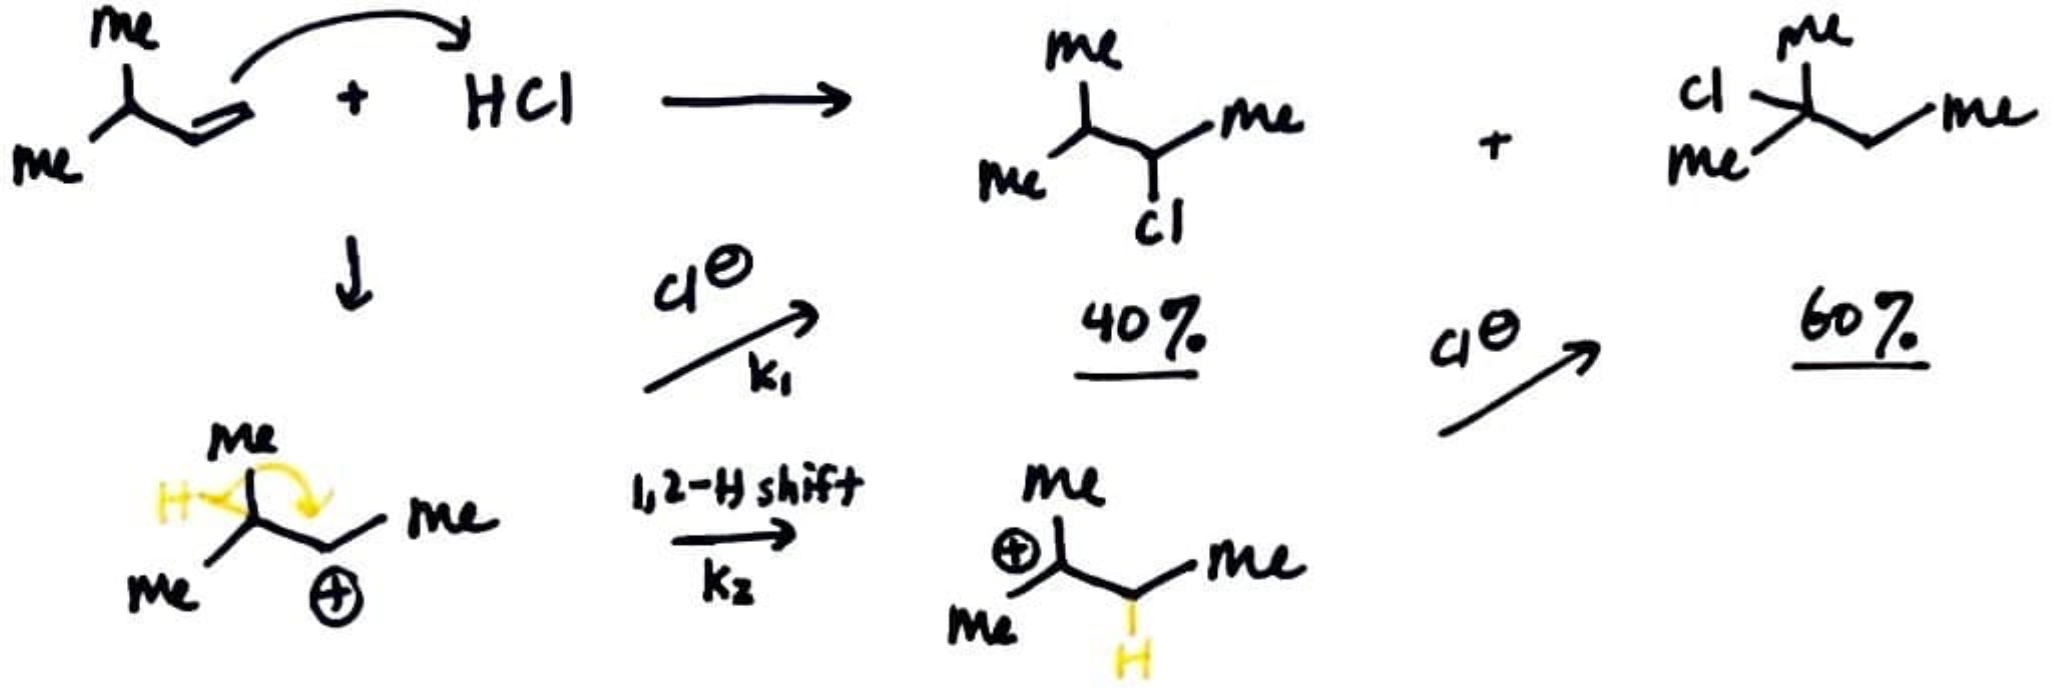
\includegraphics[width=0.6\linewidth]{HshiftHydrohalo.png}
        \caption{Hydride shifts in hydrohalogenations.}
        \label{fig:HshiftHydrohalo}
    \end{figure}
    \begin{itemize}
        \item Consider the reaction of 3-methylbut-1-ene with \ce{HCl}.
        \item We might expect the major product to be the 2-chlorinated alkene.
        \begin{itemize}
            \item This would arise from formation of the more substituted, secondary carbocation.
            \item However, this is only 40\% of the product.
        \end{itemize}
        \item However, the major product (60\%) is the 3-chlorinated species!
        \begin{itemize}
            \item This product occurs because the carbocation undergoes a 1,2-hydride shift prior to trapping by chloride.
        \end{itemize}
        \item Indeed,
        \begin{equation*}
            \frac{k_1}{k_2} = \frac{40}{60} = 0.67
        \end{equation*}
        if the $k_2$ step is irreversible.
        \item But why do we get a hydride shift instead of a methyl shift?
        \begin{itemize}
            \item Because a methyl shift would not generate a more stable carbocation! It would still be secondary.
            \item General rule: \ce{H}-shifts are better than alkyl shifts because they form more substituted carbocations.
        \end{itemize}
    \end{itemize}
    \item We now look at a case where we have to distinguish between two mechanistic possibilities that form carbocations.
    \begin{figure}[h!]
        \centering
        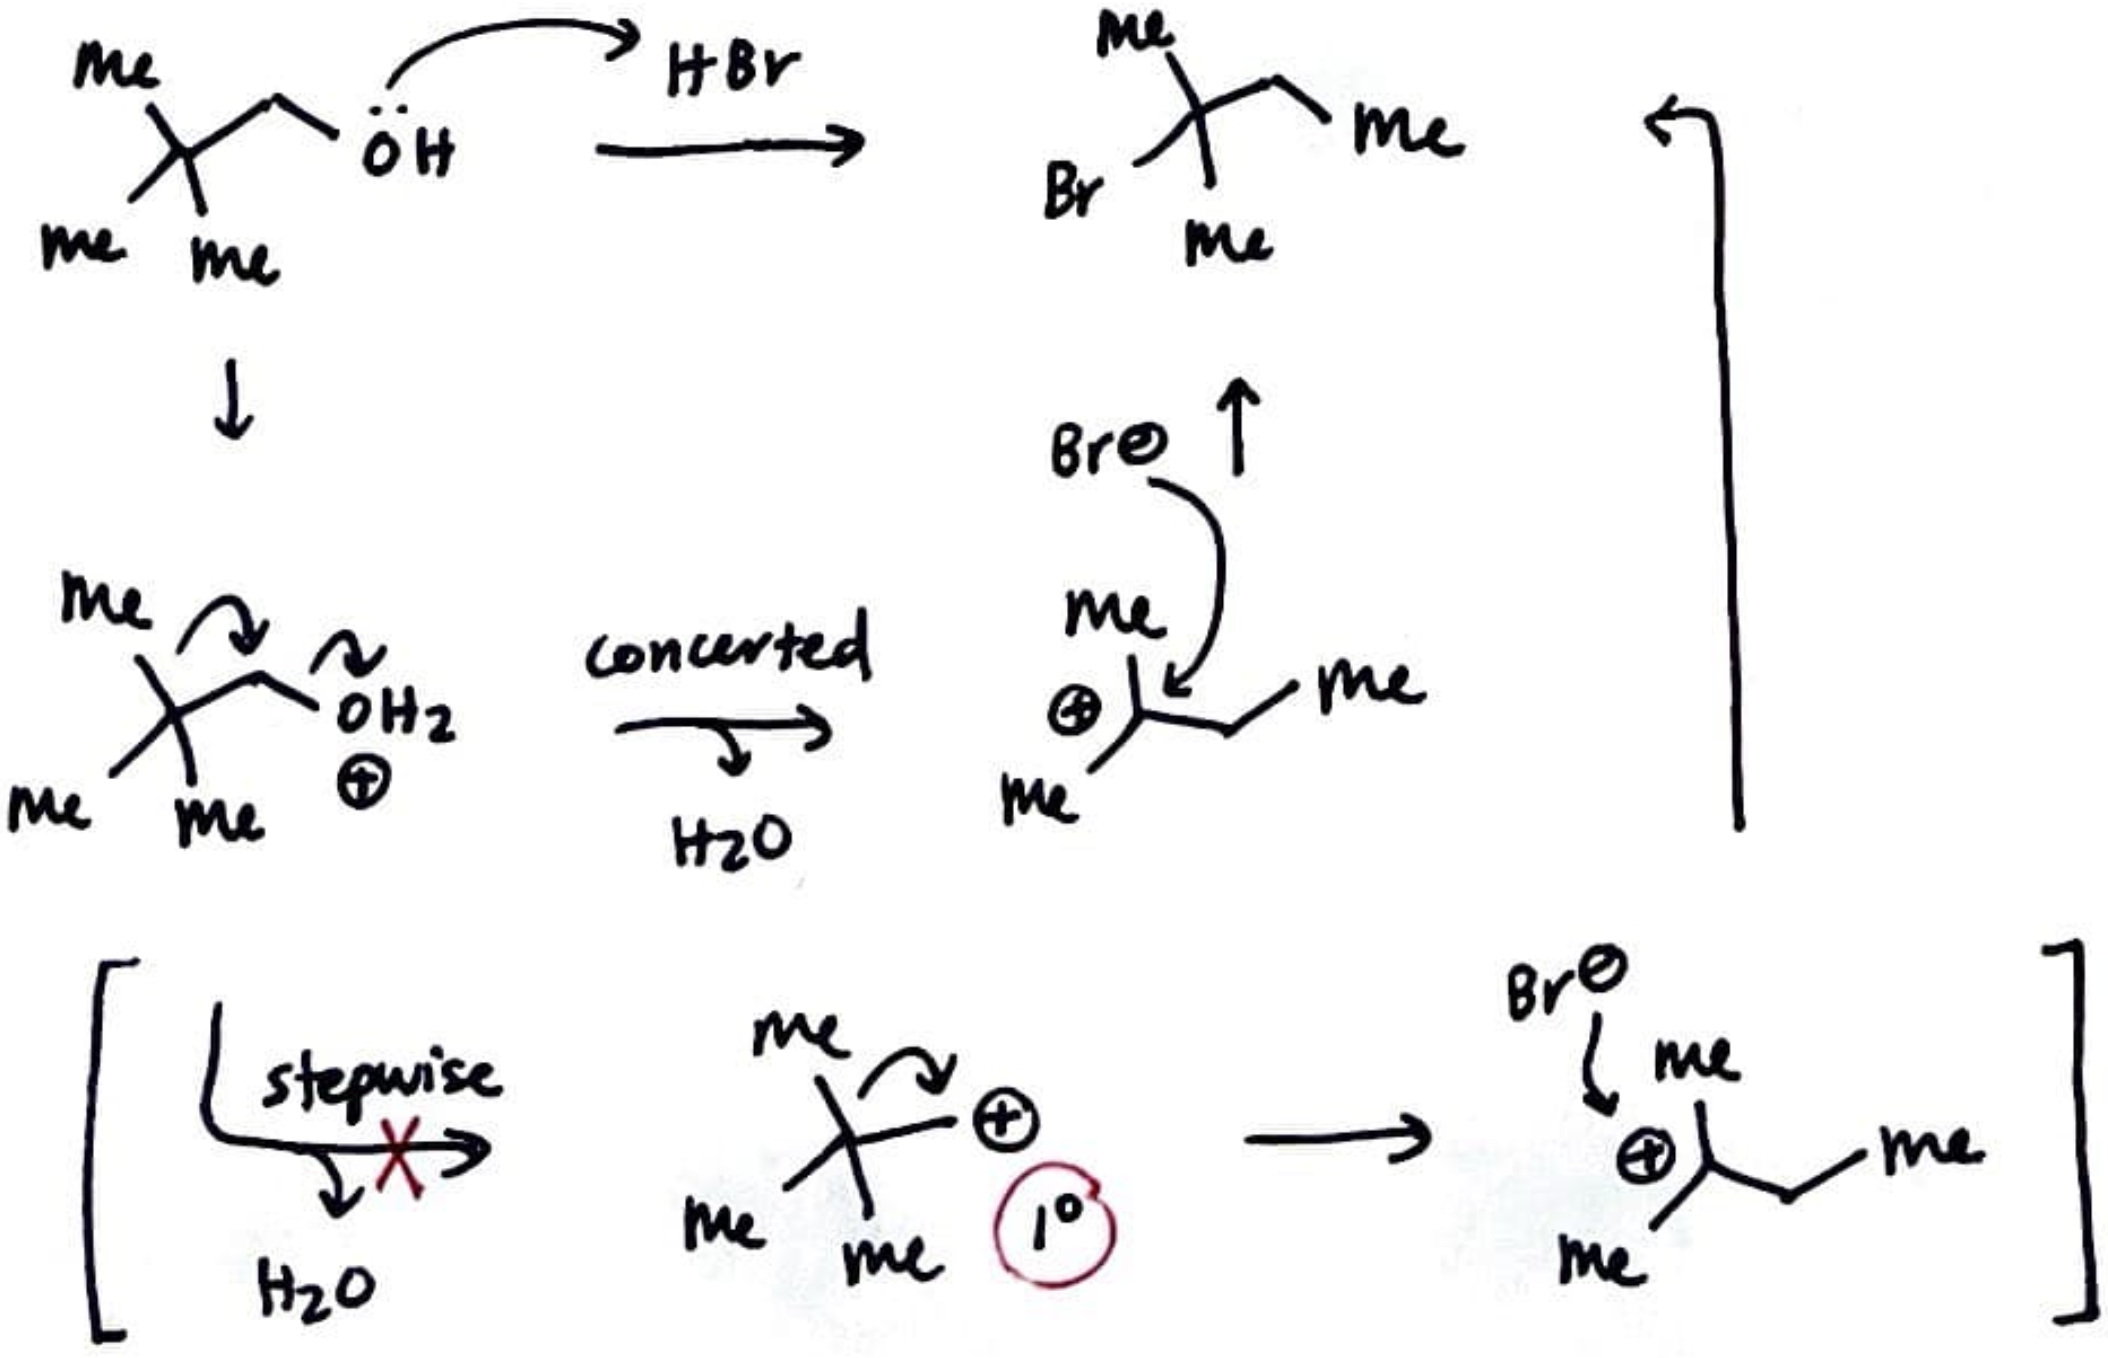
\includegraphics[width=0.6\linewidth]{concertedStepMethyl.png}
        \caption{Concerted vs. stepwise mechanisms with methyl shifts.}
        \label{fig:concertedStepMethyl}
    \end{figure}
    \begin{itemize}
        \item Consider the reaction of neopentyl alcohol with \ce{HBr}. What is the most plausible mechanism?
        \item The alcohol will get protonated and \emph{could} leave to yield a primary carbocation, which could then stepwise rearrange into a secondary cation that could be trapped.
        \begin{itemize}
            \item But we've said that in this class, primary carbocations are not allowed!
        \end{itemize}
        \item Thus, we can make use of a concerted pathway (Figure \ref{fig:CCrearrb}).
        \begin{itemize}
            \item This mechanism affords the secondary carbocation directly, which can then react.
        \end{itemize}
        \item Thinking about the relative energies of competing transition states is useful here.
    \end{itemize}
    \pagebreak
    \item Chemists love small rings; let's look at a strain-releasing reaction with them.
    \begin{figure}[h!]
        \centering
        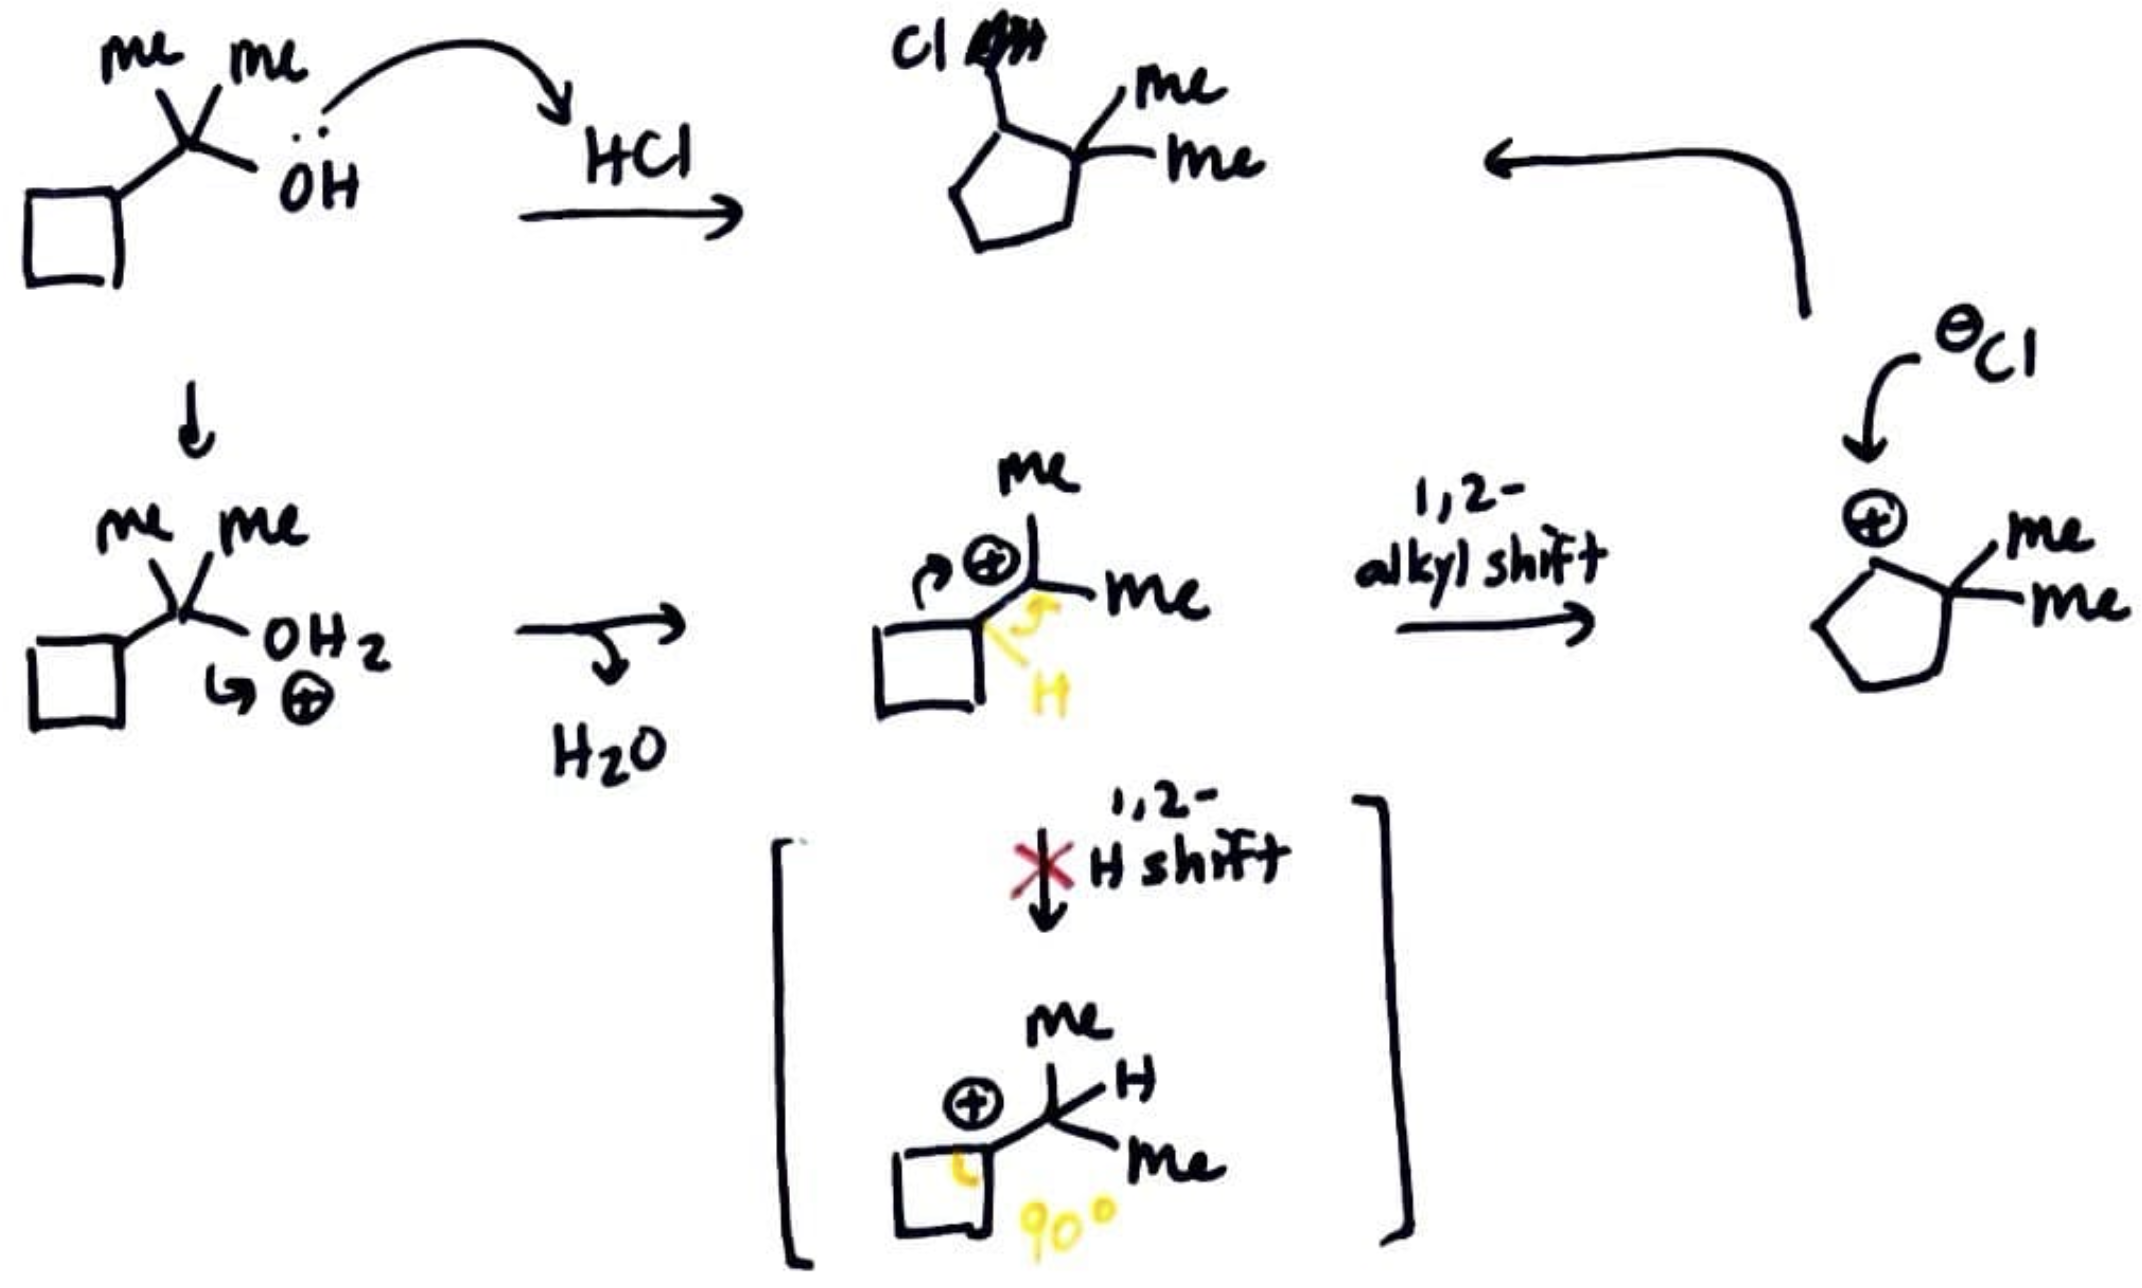
\includegraphics[width=0.6\linewidth]{angleStrainAlk.png}
        \caption{Angle strain can induce alkyl shifts.}
        \label{fig:angleStrainAlk}
    \end{figure}
    \begin{itemize}
        \item Consider the reaction of 2-cyclobutylpropan-2-ol with \ce{HCl}.
        \item If we form the tertiary carbocation and then do an \ce{H}-shift to put the cation in the 4-membered ring, we will induce immense strain.
        \begin{itemize}
            \item $sp^2$ likes to be \ang{120}, and we've got it confined to \ang{60}!
        \end{itemize}
        \item Instead, we can do an alkyl shift to release strain, even though it forms a secondary carbocation.
        \item Takeaway: In cases where all else is equal, prefer \ce{H}-shifts. But there do exist cases in which all else is \emph{not} equal!
    \end{itemize}
    \item Let's now look at some rearrangements.
    \begin{itemize}
        \item We're going to teach 7-10 rearrangements that involve carbocation intermediates.
        \item You can probably find another 500 if you go looking; most will have somebody's name on them.
    \end{itemize}
    \item Dienone-phenol rearrangement.
    \begin{figure}[h!]
        \centering
        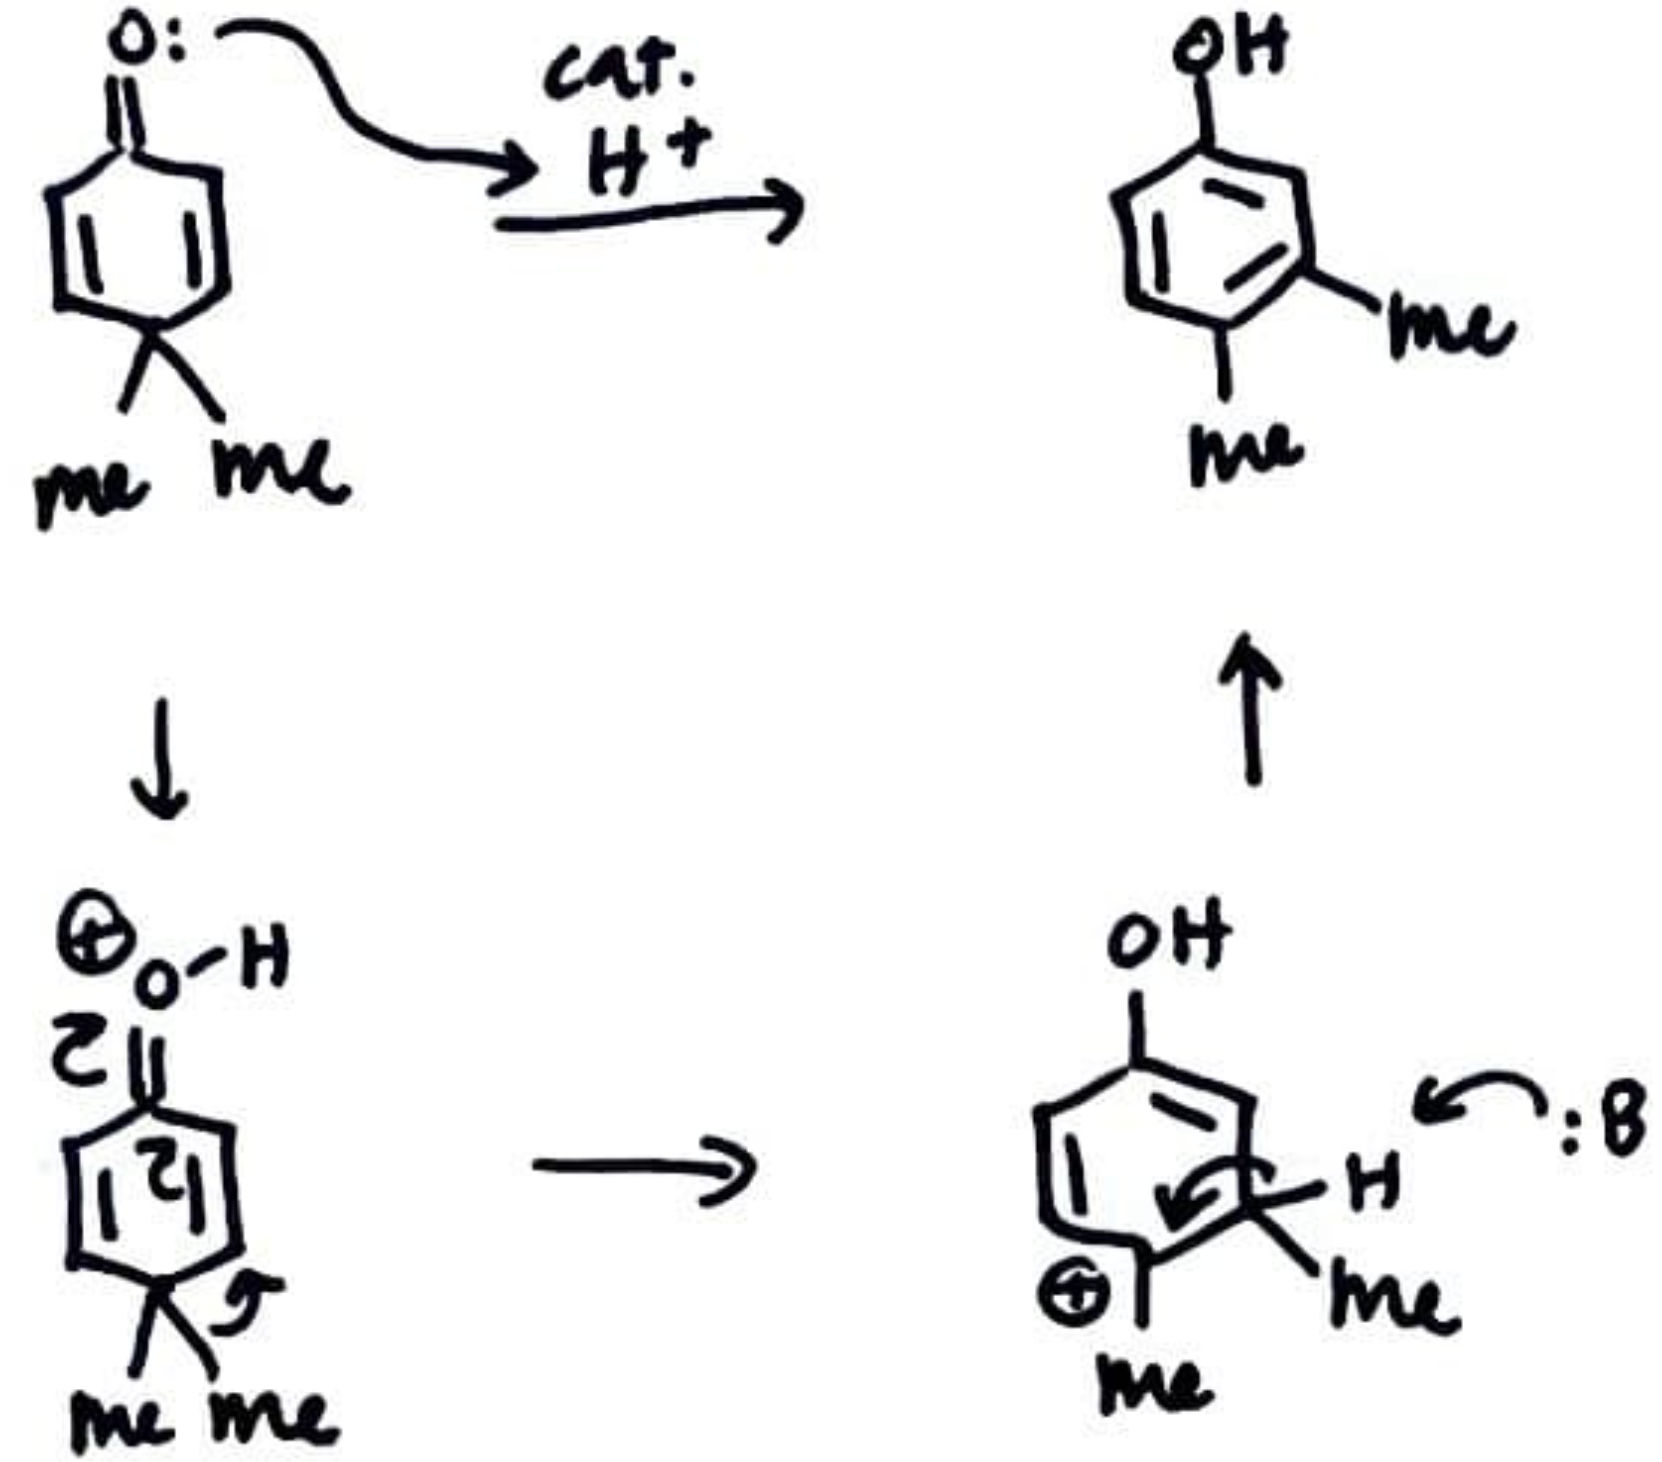
\includegraphics[width=0.4\linewidth]{dienonePhenol.png}
        \caption{Dienone-phenol rearrangement.}
        \label{fig:dienonePhenol}
    \end{figure}
    \pagebreak
    \begin{itemize}
        \item If we didn't have blocking methyl groups, we would tautomerize to the fully aromatic system.
        \item But in the presence of catalytic acid, we get 3,4-dimethylphenol!
        \item Protonating the carbonyl makes the $\beta$-positions \emph{very, very} electron-deficient; consider the enol resonance structure!
        \begin{itemize}
            \item Thus, a 1,2-migration can give us a stabilized tertiary, allylic carbocation.
        \end{itemize}
        \item Then some group (doesn't have to be very basic) can come in to deprotonate and aromatize the system.
    \end{itemize}
    \item TTQ: What happens to this the species at top-left below in the presence of acid?
    \begin{figure}[h!]
        \centering
        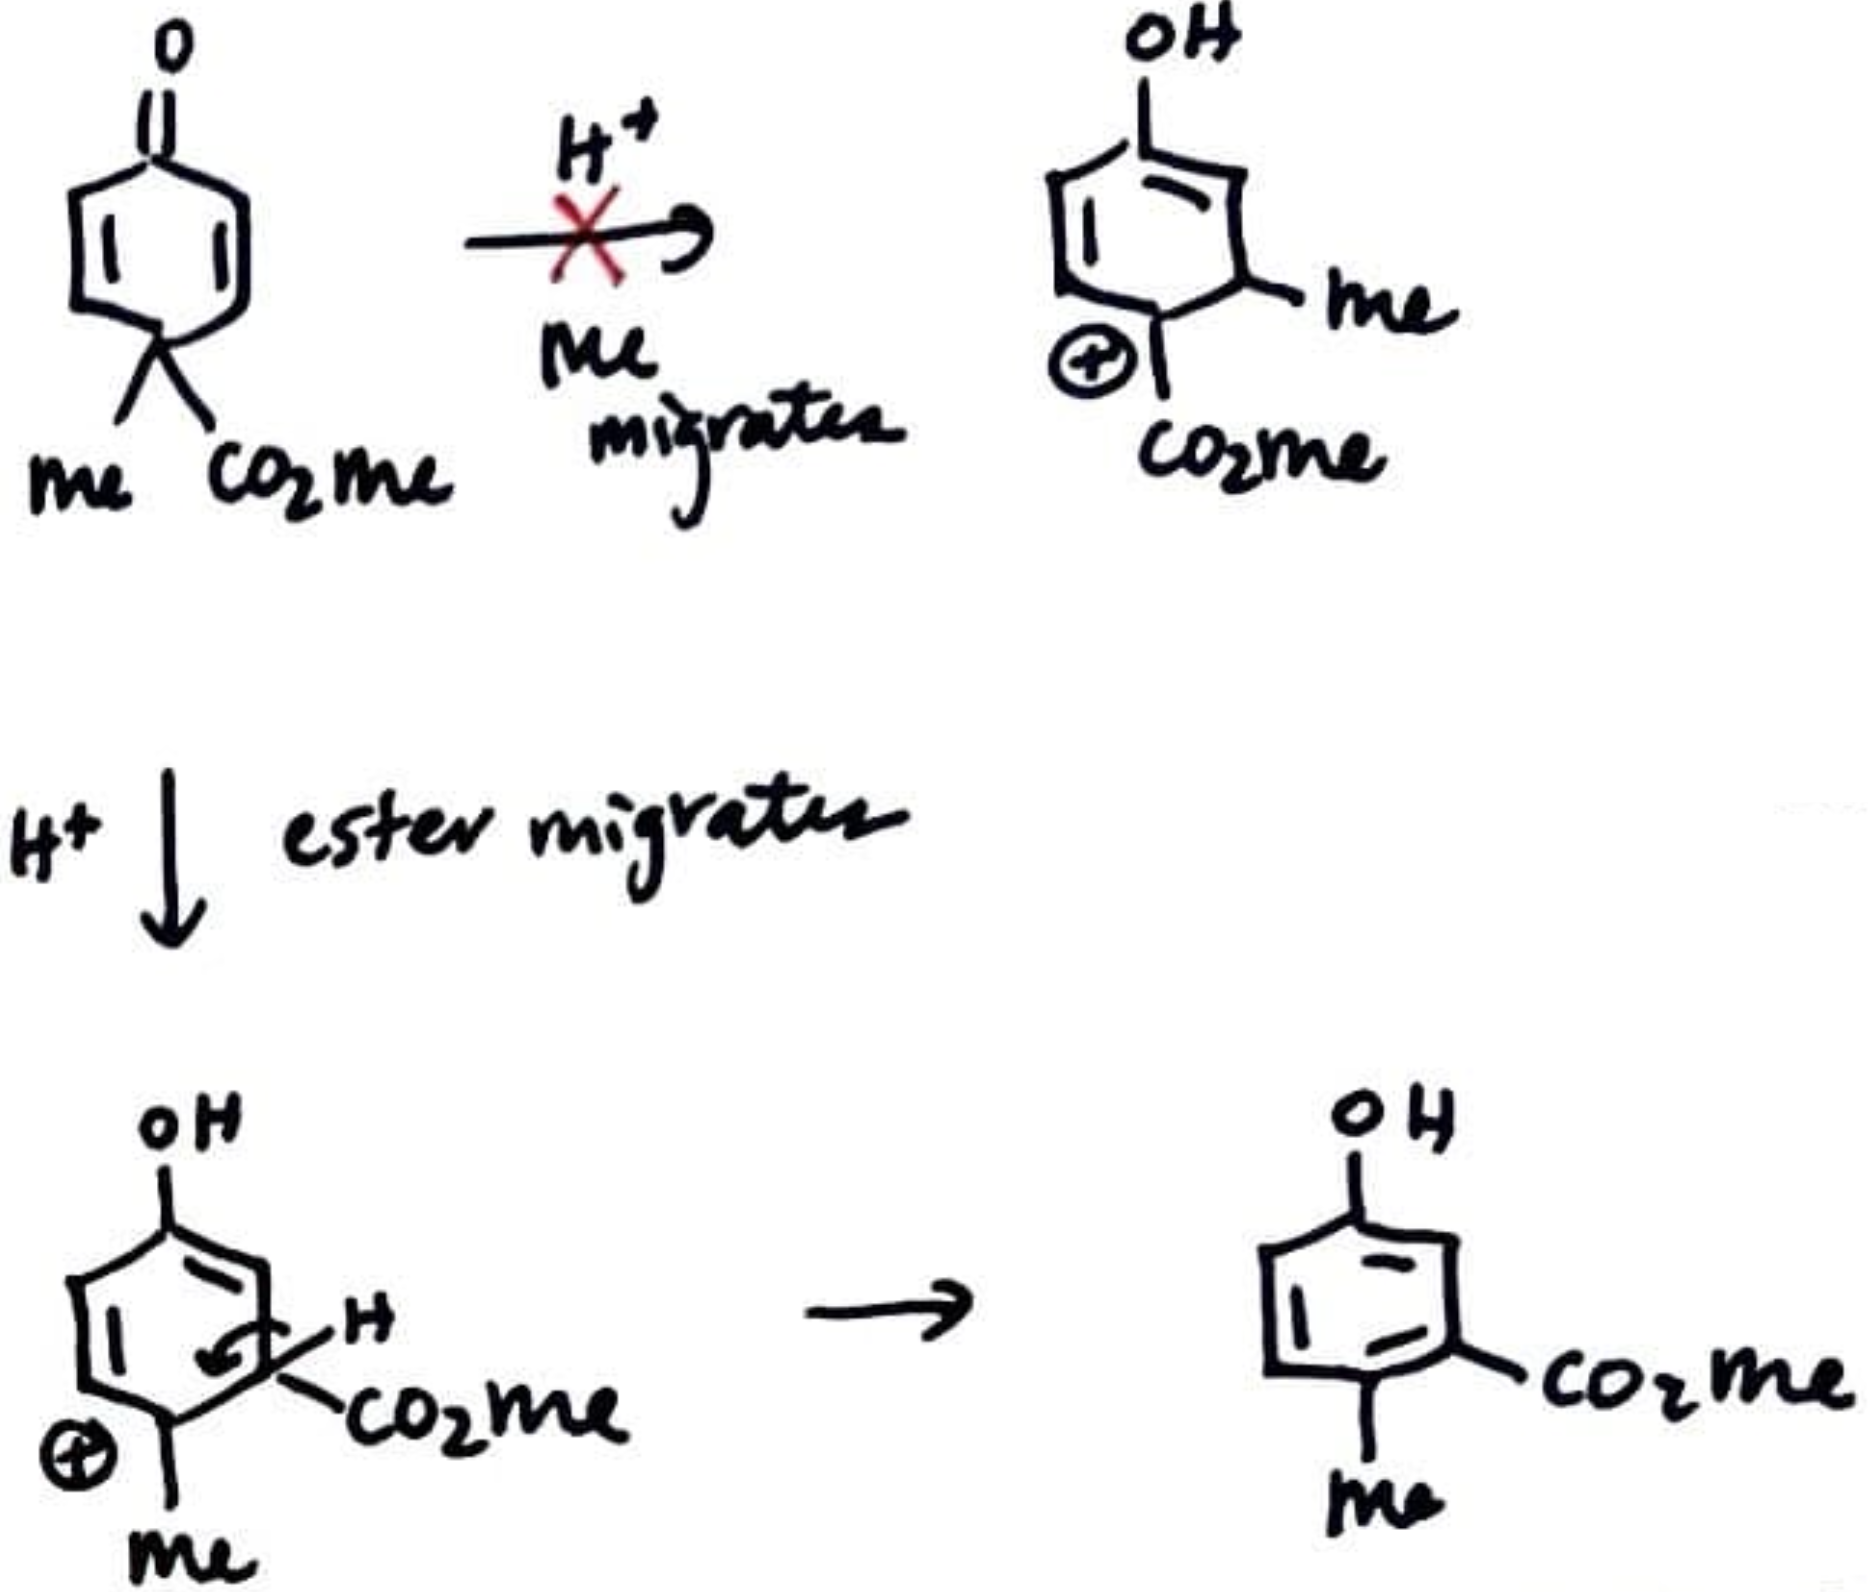
\includegraphics[width=0.35\linewidth]{TTQesterShift.png}
        \caption{TTQ: Ester shifts.}
        \label{fig:TTQesterShift}
    \end{figure}
    \begin{itemize}
        \item Two things can happen: Either the methyl group or the ester group can migrate.
        \item However, having the carbocation be next to a methyl group is far more favorable than having it next to a destabilizing EWG like an ester.
        \item Thus, the reaction proceeds via an ester shift to yield the drawn phenol!
    \end{itemize}
    \item Converting epoxides to aldehydes.
    \begin{figure}[h!]
        \centering
        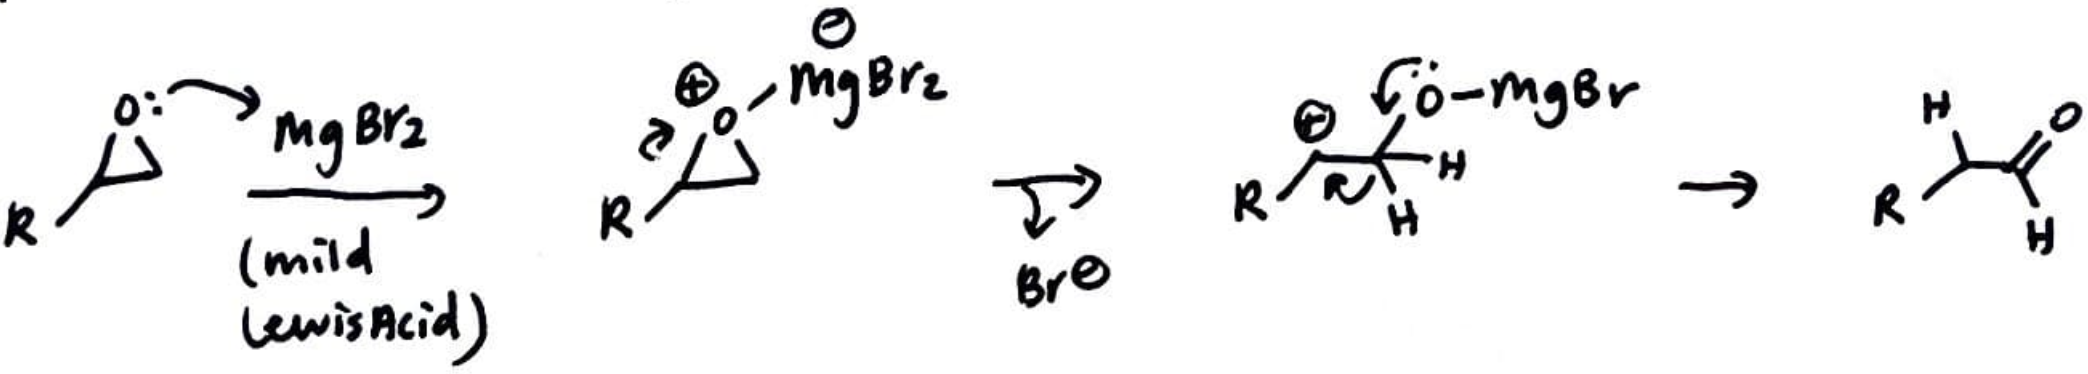
\includegraphics[width=0.7\linewidth]{epoxideAldehydeRearr.png}
        \caption{Epoxide-aldehyde rearrangement.}
        \label{fig:epoxideAldehydeRearr}
    \end{figure}
    \begin{itemize}
        \item \ce{MgBr2} is a mild Lewis acid that will coordinate to the epoxide oxygen.
        \item The epoxide can then open, formally bonding to magnesium and kicking out one bromide.
        \item The \ce{O-Mg} bond then collapses into the forming aldehyde $\pi$-system with a concurrent 1,2-\ce{H} shift.
    \end{itemize}
    \item Synthetic utility of the epoxide-aldehyde rearrangement.
    \begin{figure}[H]
        \centering
        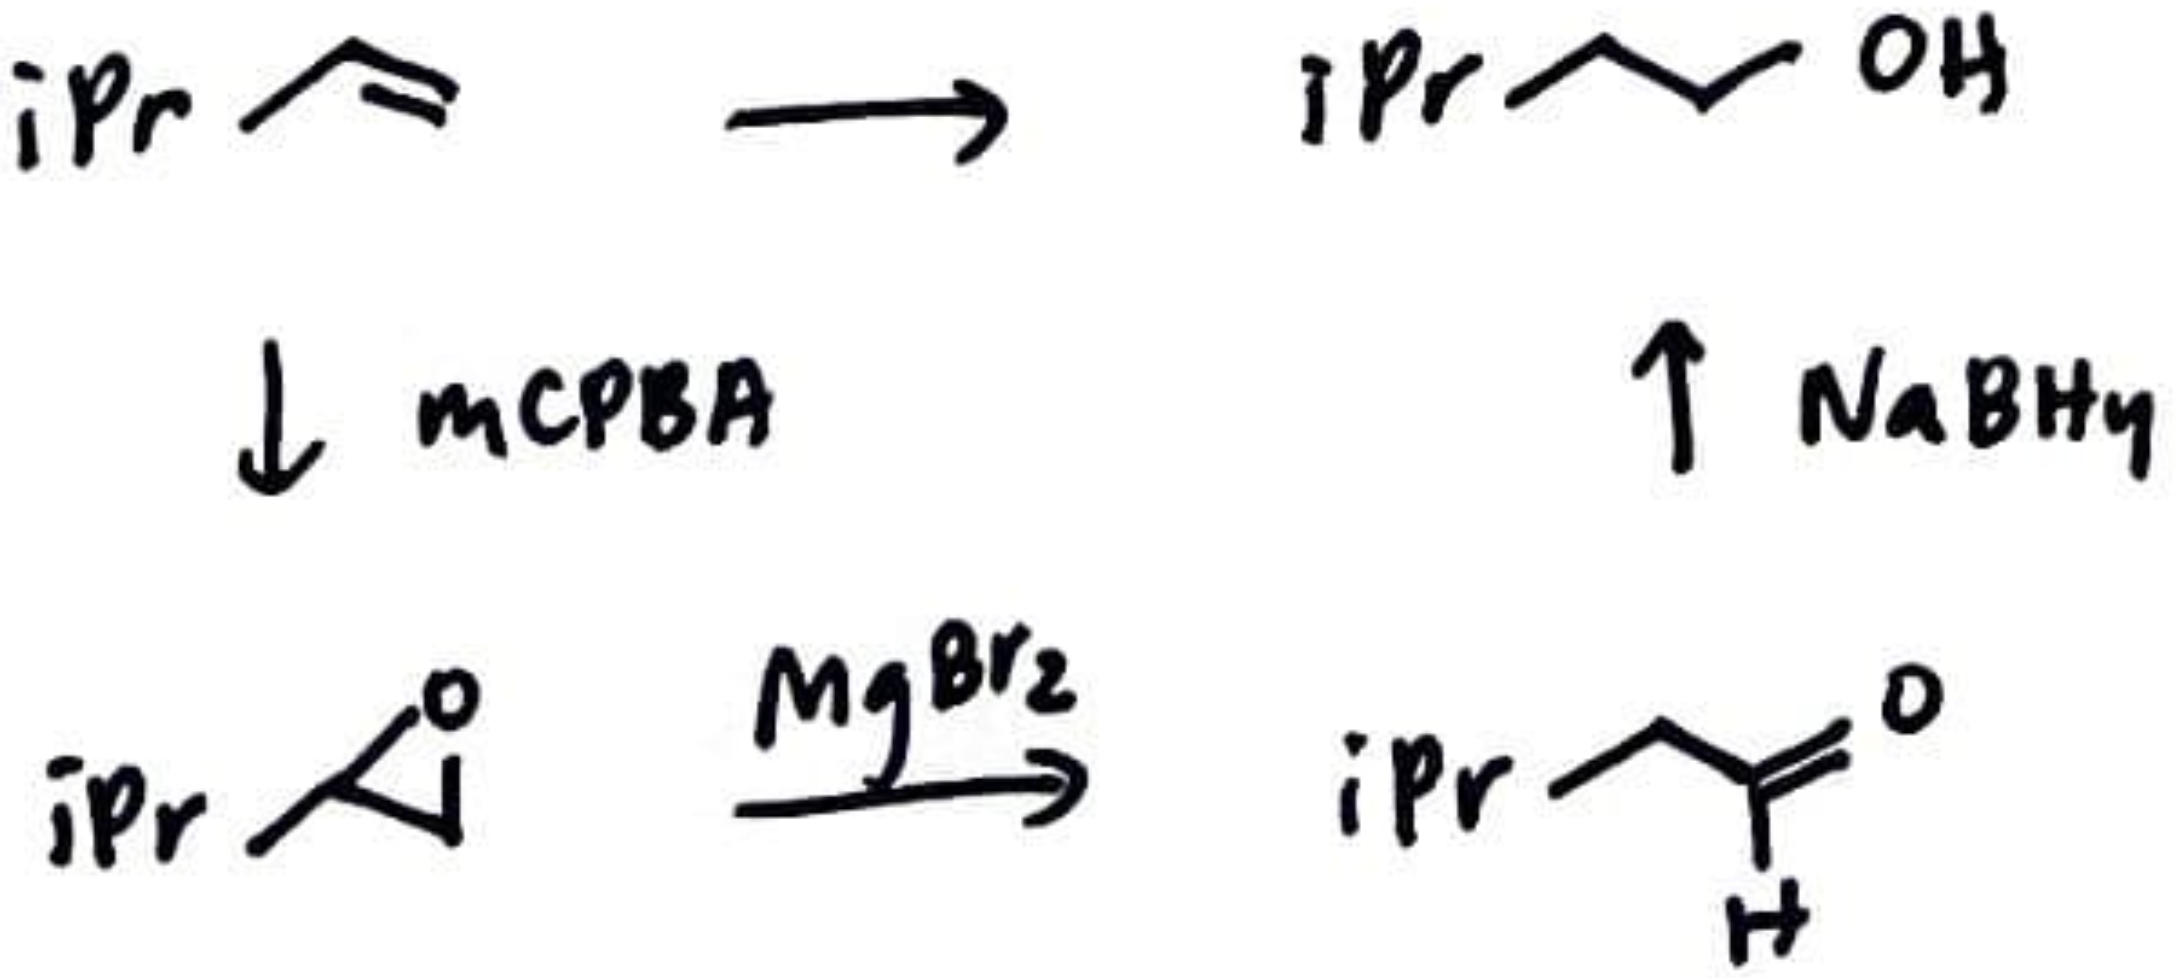
\includegraphics[width=0.3\linewidth]{epoxideAldehydeRearrUse.png}
        \caption{Epoxide-aldehyde rearrangement: Synthetic utility.}
        \label{fig:epoxideAldehydeRearrUse}
    \end{figure}
    \begin{itemize}
        \item We start with an alkene, turn it into an epoxide, open it as in Figure \ref{fig:epoxideAldehydeRearr}, and then reduce it.
        \item This is an alternative to hydroboration!
    \end{itemize}
    \item Alternatives are important as they can be safer, cleaner, and more generally applicable to complicated systems.
    \begin{itemize}
        \item Both Profs. Buchwald and Elkin research such reaction alternatives in their labs!
    \end{itemize}
    \item Pinacol rearrangement of 1,2-diols.
    \begin{figure}[h!]
        \centering
        \begin{subfigure}[b]{\linewidth}
            \centering
            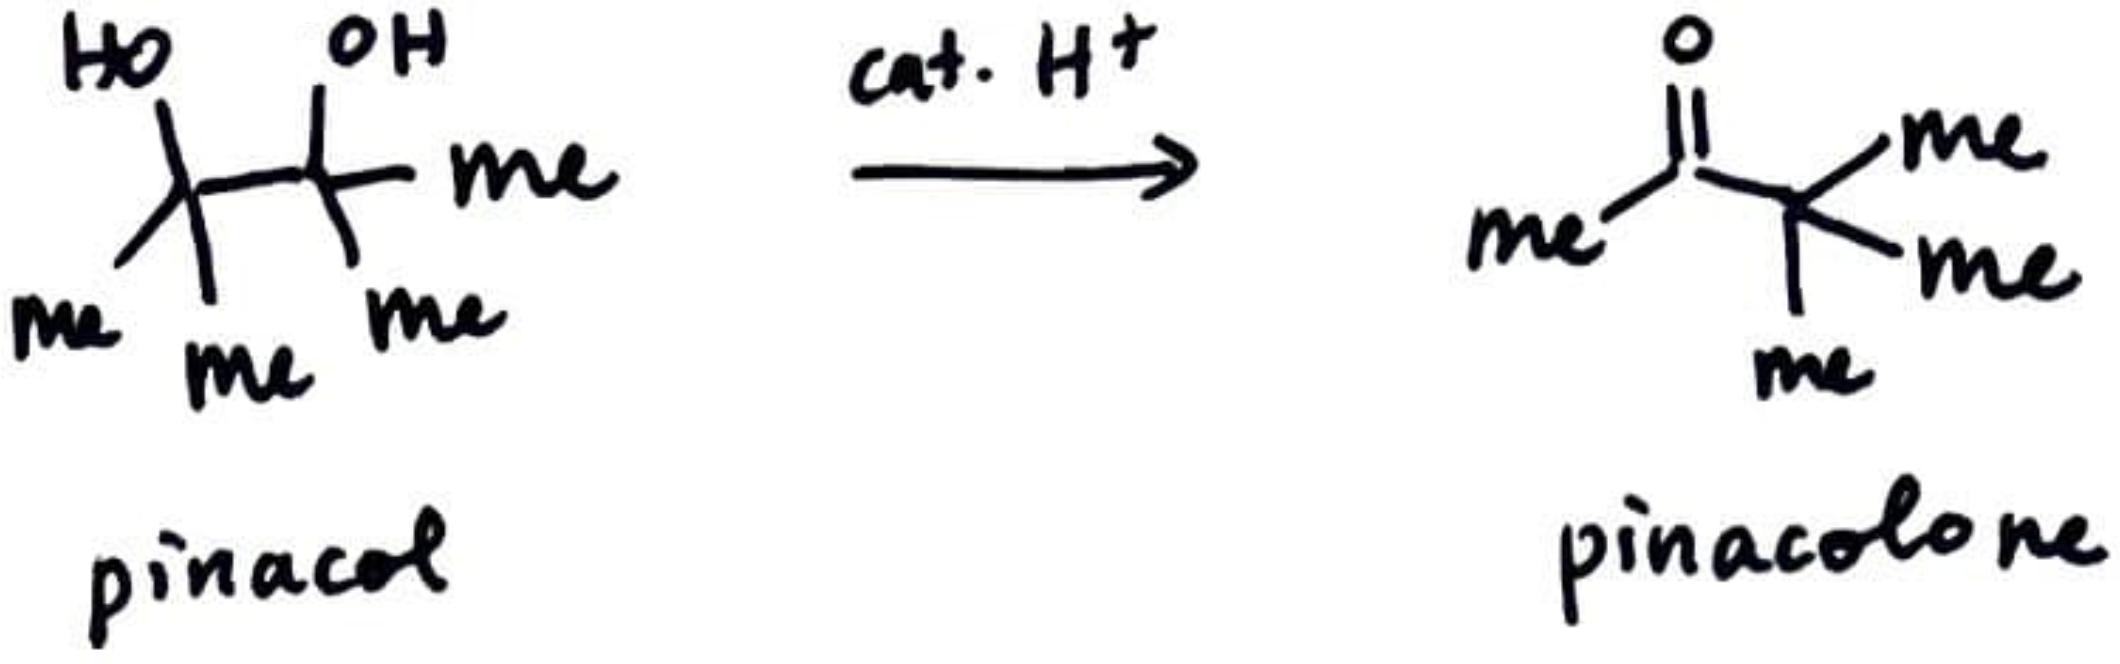
\includegraphics[width=0.4\linewidth]{pinacolPinacolonea.png}
            \caption{General form.}
            \label{fig:pinacolPinacolonea}
        \end{subfigure}\\[2em]
        \begin{subfigure}[b]{\linewidth}
            \centering
            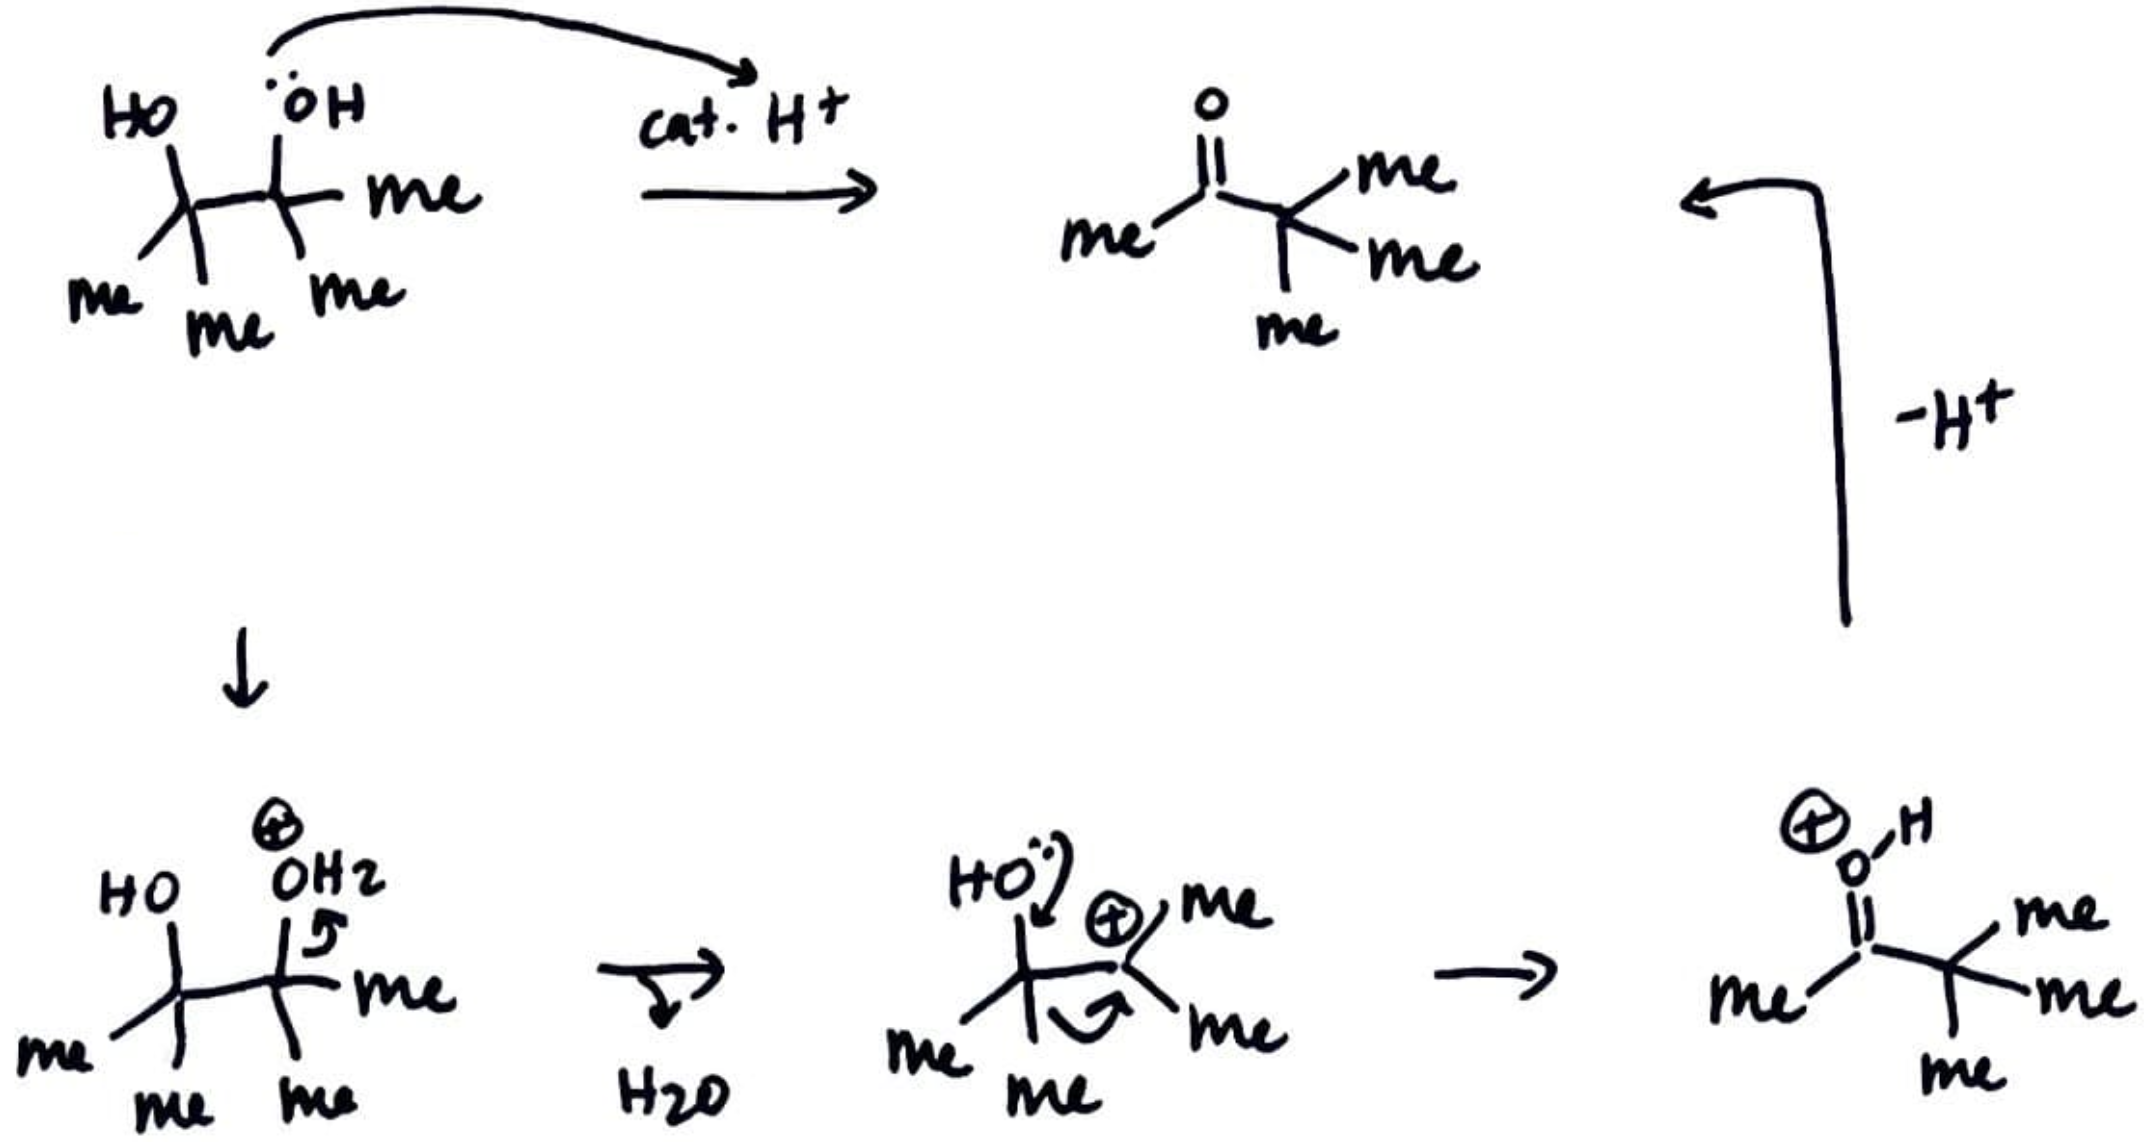
\includegraphics[width=0.6\linewidth]{pinacolPinacoloneb.png}
            \caption{Mechanism.}
            \label{fig:pinacolPinacoloneb}
        \end{subfigure}
        \caption{Pinacol-pinacolone rearrangement.}
        \label{fig:pinacolPinacolone}
    \end{figure}
    \begin{itemize}
        \item Mechanistically, we begin by protonating a hydroxyl group to form a good leaving group.
        \item Then we get a rearrangement, thermodynamically driven by the formation of a carbonyl.
        \item Final deprotonation yields the pinacolone product.
    \end{itemize}
    \item Asymmetric pinacol rearrangements.
    \begin{figure}[H]
        \centering
        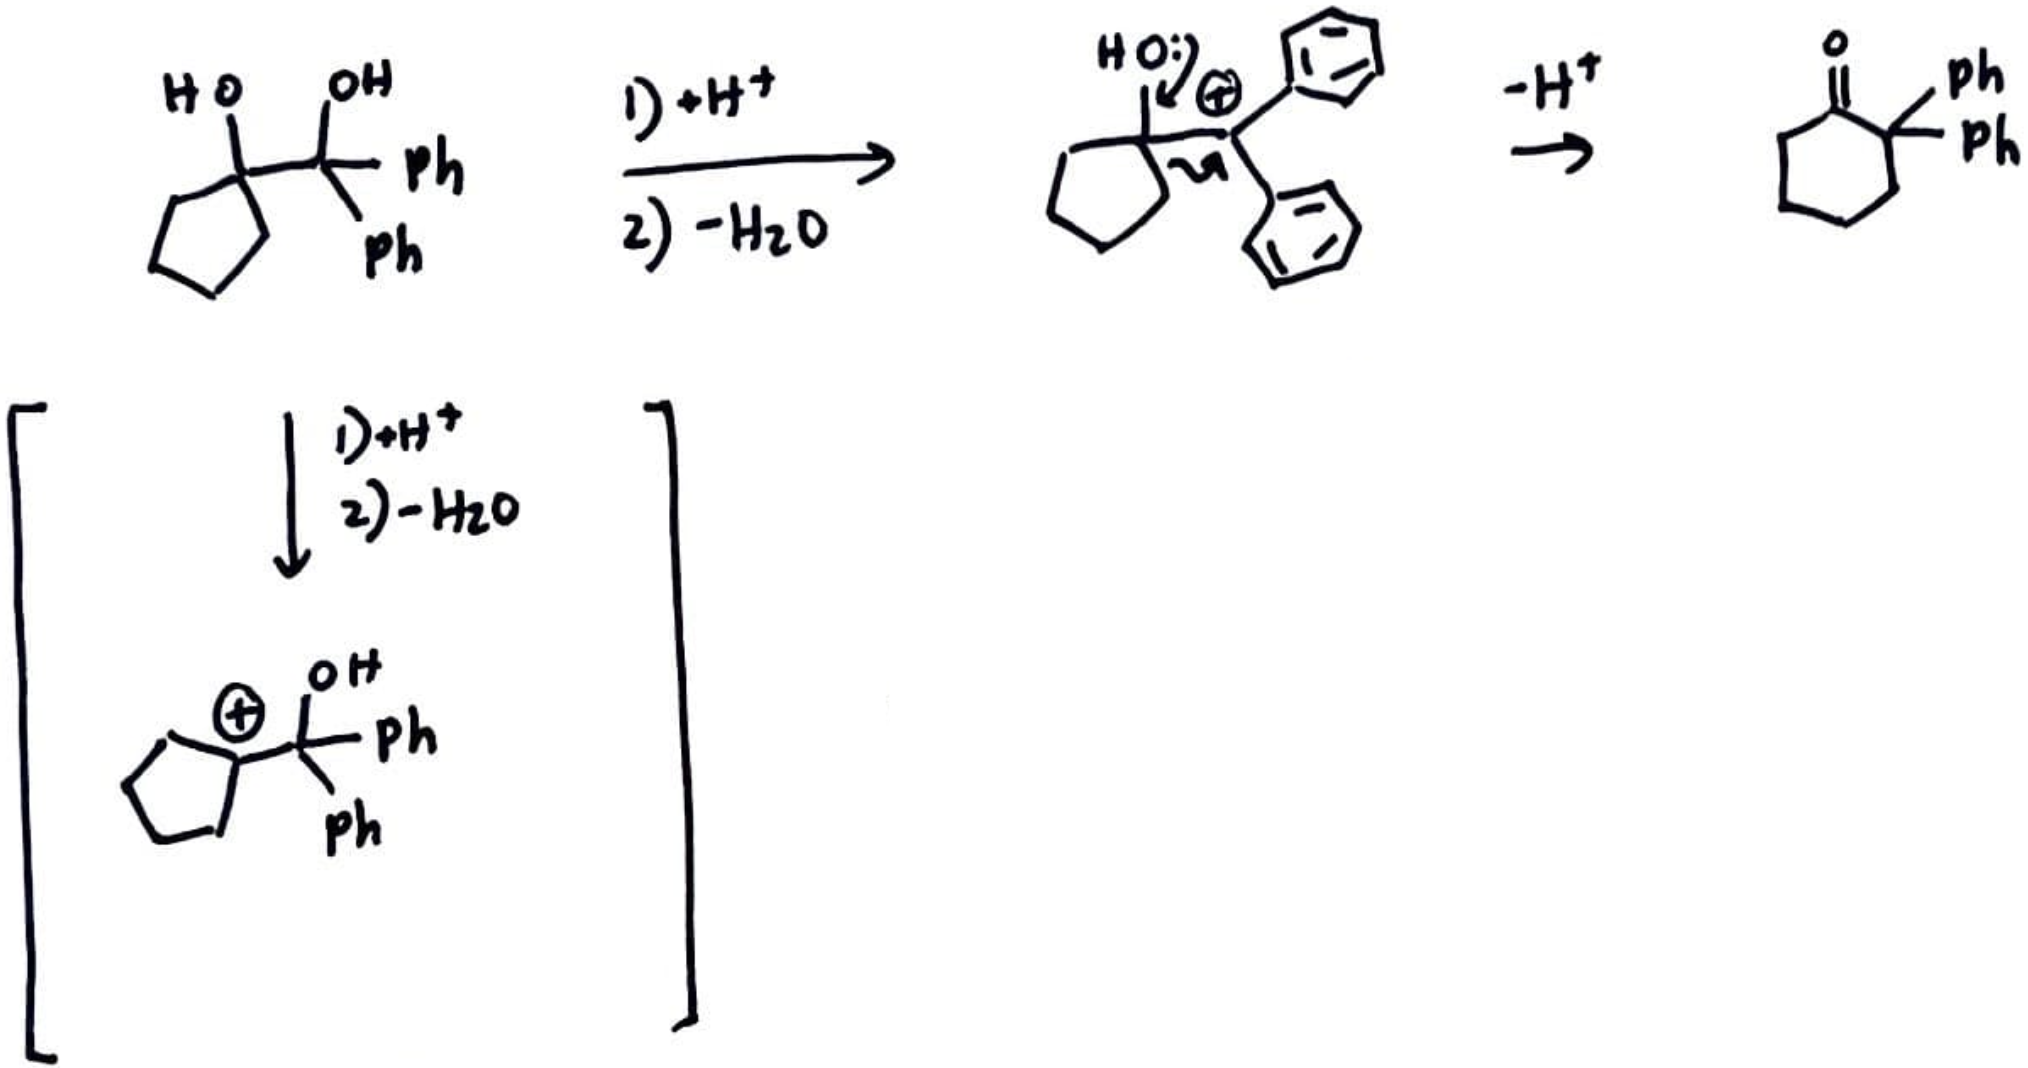
\includegraphics[width=0.6\linewidth]{pinacolPinacoloneAsy.png}
        \caption{Asymmetric pinacol-pinacolone rearrangement.}
        \label{fig:pinacolPinacoloneAsy}
    \end{figure}
    \begin{itemize}
        \item Both possible carbocations we could form from this substrate are quite good!
        \begin{itemize}
            \item However, while the tertiary carbocation is good, the tertiary diphenyl carbocation is \emph{awesome}; it should be in the carbocation hall of fame!
        \end{itemize}
        \item Thus, we get another alkyl shift, yielding a product with a six-membered ring.
    \end{itemize}
    \item Baeyer-Villiger oxidation.
    \begin{figure}[h!]
        \centering
        \begin{subfigure}[b]{\linewidth}
            \centering
            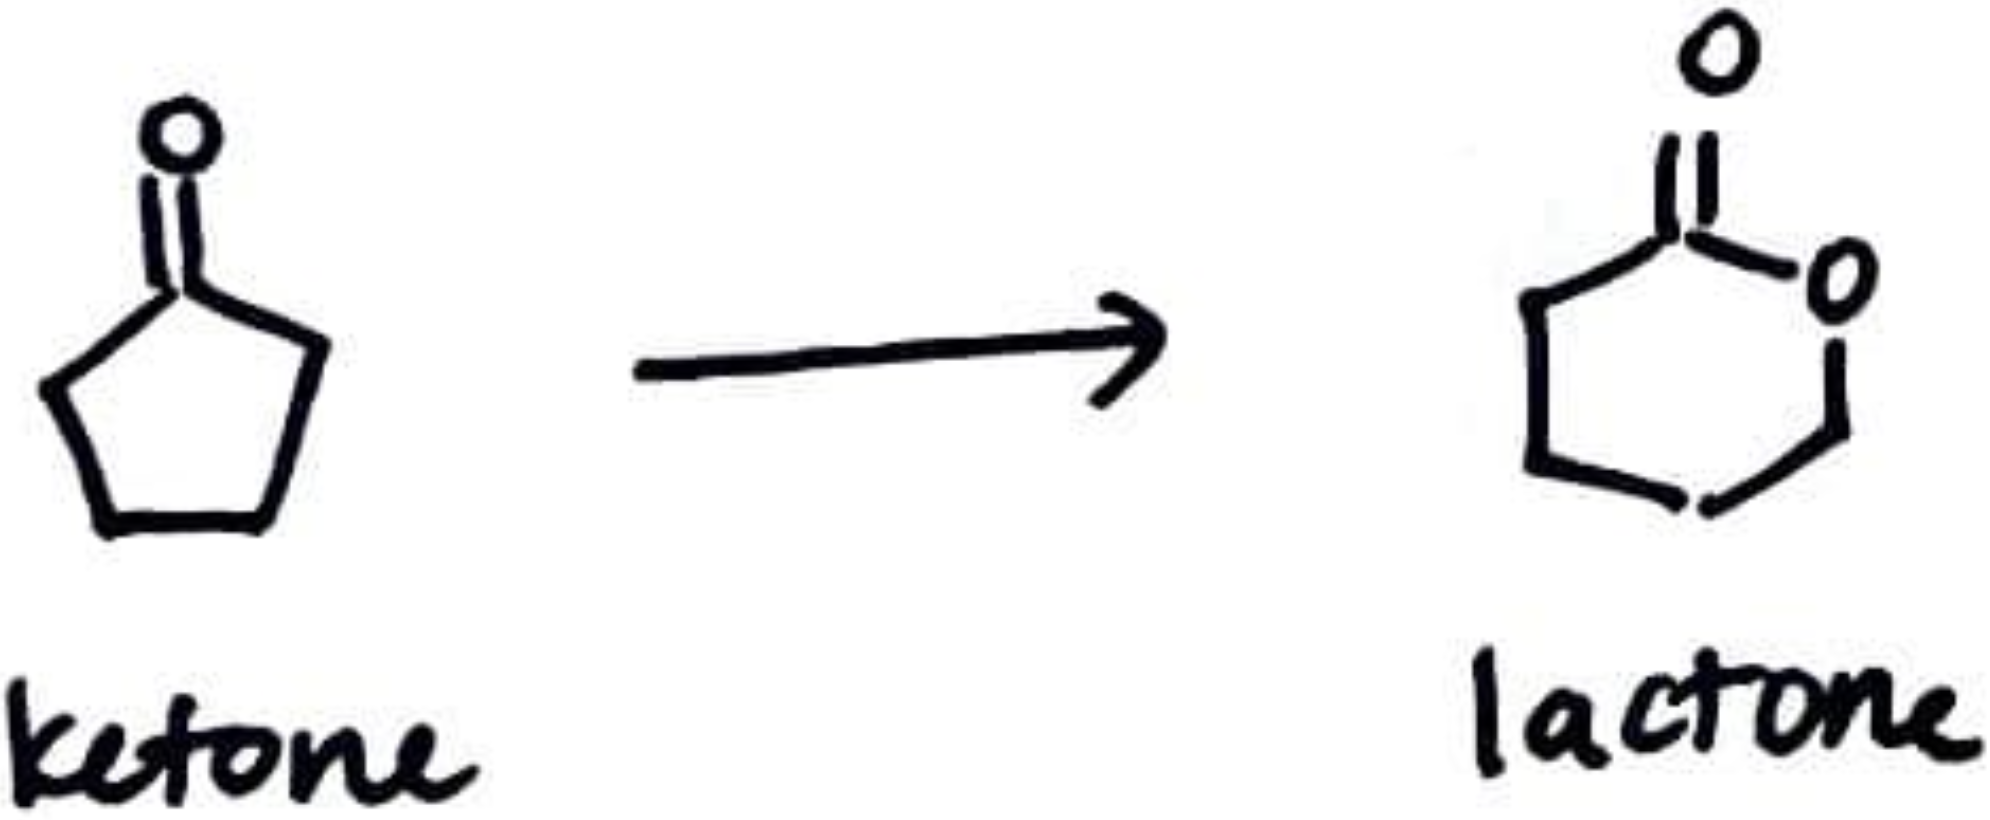
\includegraphics[width=0.25\linewidth]{BaeyerVilligera.png}
            \caption{General form.}
            \label{fig:BaeyerVilligera}
        \end{subfigure}\\[2em]
        \begin{subfigure}[b]{\linewidth}
            \centering
            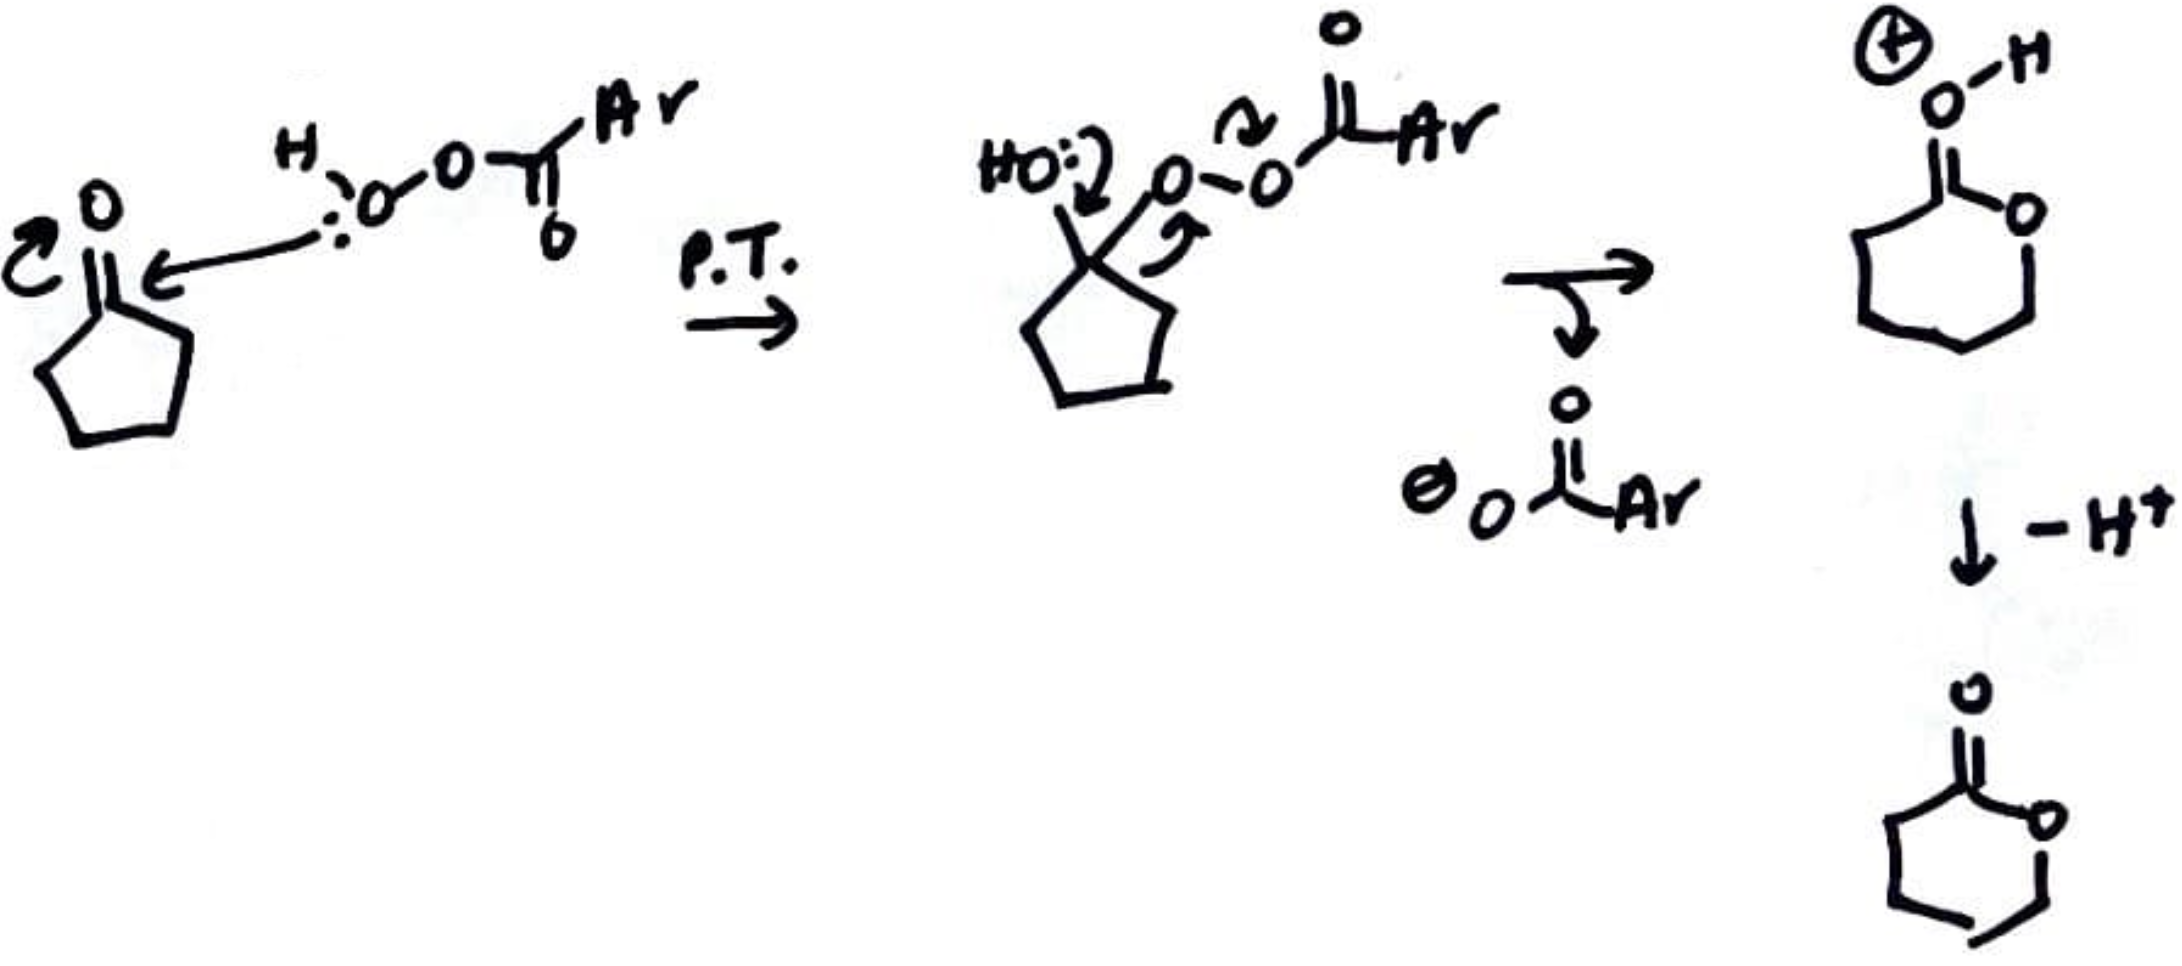
\includegraphics[width=0.5\linewidth]{BaeyerVilligerb.png}
            \caption{Mechanism.}
            \label{fig:BaeyerVilligerb}
        \end{subfigure}
        \caption{Baeyer-Villiger oxidation.}
        \label{fig:BaeyerVilliger}
    \end{figure}
    \begin{itemize}
        \item Here, we convert a ketone into a lactone.
        \item We generally use a peracid (like \emph{m}CPBA) to make this reaction proceed.
        \begin{itemize}
            \item We can just use a peroxide sometimes, though.
        \end{itemize}
        \item There's a very good depiction of the mechanism on \textcite[956]{bib:Clayden}.
    \end{itemize}
    \item Regioselectivity of the Baeyer-Villiger oxidation.
    \begin{figure}[h!]
        \centering
        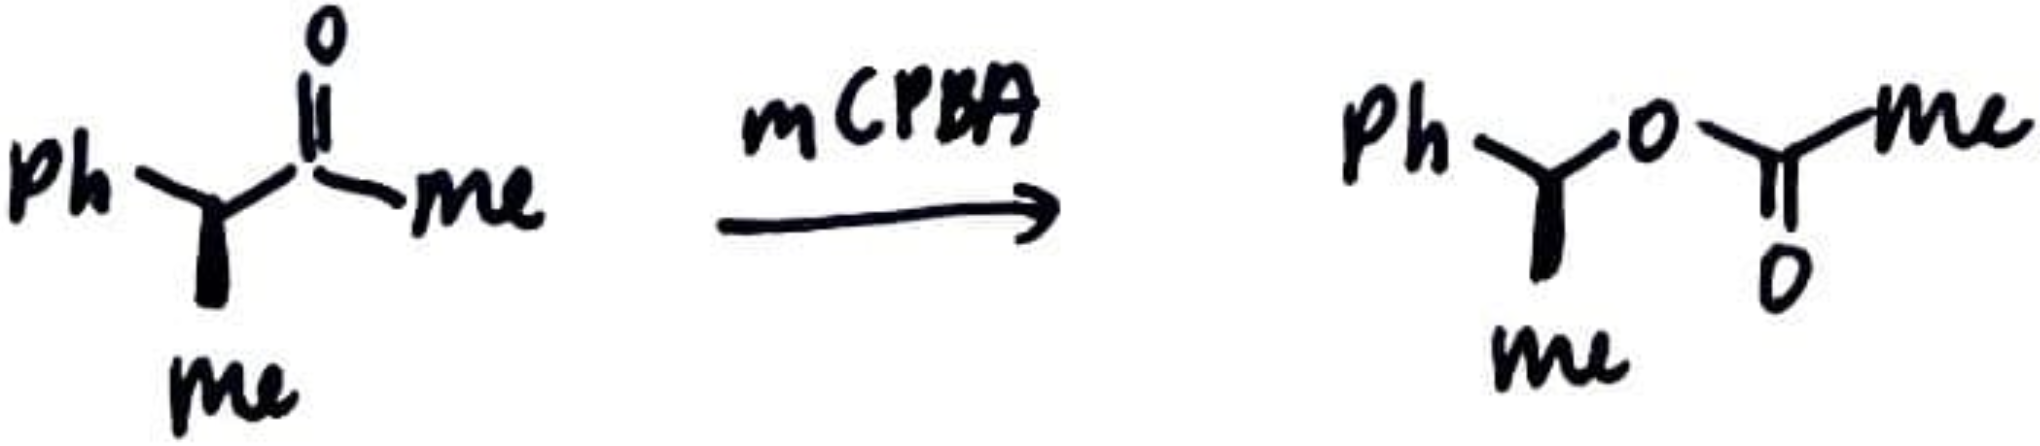
\includegraphics[width=0.4\linewidth]{BaeyerVilligerRegio.png}
        \caption{Baeyer-Villiger oxidation regioselectivity.}
        \label{fig:BaeyerVilligerRegio}
    \end{figure}
    \begin{itemize}
        \item The example in Figure \ref{fig:BaeyerVilliger} was symmetric, but what if our ketone is asymmetric?
        \item Here, we get exclusively the drawn enantiopure product from the drawn enantiopure starting material.
        \item To decide regioselectivity, consider the migratory aptitude of various groups.
        \begin{equation*}
            3^\circ > 2^\circ > \text{phenyl} > \ce{Me}
        \end{equation*}
        \begin{itemize}
            \item The drawing on \textcite[956]{bib:Clayden} has a good rationalization for this!
            \item The typical rationalization is for which can best stabilize a positive charge; note that phenyl is the odd one out because it's weird.
            \item Vinyl is not included because double bonds in the presence of \emph{m}CPBA will lead to an epoxidation more rapidly than a Baeyer-Villiger.
        \end{itemize}
        \item Thus, we form the drawn product because a $2^\circ$ carbons migrates instead of a methyl group.
    \end{itemize}
\end{itemize}




\end{document}